\renewcommand{\theequation}{\theenumi}
\renewcommand{\thefigure}{\theenumi}
\begin{enumerate}[label=\thesubsection.\arabic*.,ref=\thesubsection.\theenumi]
\numberwithin{equation}{enumi}
\numberwithin{figure}{enumi}
%
\item Prove that the following equations represent two straight lines, find also their point of intersection and the angle between them.\\
$6y^2-xy-x^2+30y+36=0$.
%
\\
\solution

The given equation can be written as:
\begin{align}
-x^2-xy+6y^2+30y+36=0 \label{eq:solutions/13/1/eq1}
\end{align}
\mydet{\vec{V}&\vec{u}\\\vec{u}^T&f} of \eqref{eq:solutions/13/1/eq1} becomes
\begin{align}
    \mydet{-1&-\frac{1}{2}&0\\\frac{-1}{2}&6&15\\0&15&36}=0\label{eq:solutions/13/1/eq02}
\end{align}
Expanding equation \eqref{eq:solutions/13/1/eq02}, we get zero.\\
Hence given equation represents a pair of straight lines.

The general equation second degree is given by
\begin{equation}\label{eq:solutions/13/1/eq5}
	ax^2 + 2bxy + cy^2 + 2dx + 2ey + f = 0
\end{equation}
Let $(\alpha,\beta)$ be their point of intersection, then
\begin{equation}\label{eq:solutions/13/1/eq6}
	\myvec{ a & h\\ h & b}\myvec{\alpha \\ \beta} = \myvec{-d \\ -e}
\end{equation}
Given equation is
\begin{align}
	-x^2-xy+6y^2+30y+36=0
\end{align}
Substituting in \eqref{eq:solutions/13/1/eq6}
\begin{align}
	\label{eq:solutions/13/1/eq16}\myvec{ -1 & \frac{-1}{2}\\\frac{-1}{2} & 6}\myvec{\alpha \\ \beta} = \myvec{0 \\ -15} \\
	\label{eq:solutions/13/1/eq17}\implies \myvec{\alpha \\ \beta} =\myvec{\frac{6}{5} \\ \frac{-12}{5}}
\end{align}
\text{Hence, the intersection point is}
\myvec{\frac{6}{5}\\-\frac{12}{5}}\\
Also, Verified using python code from
\begin{lstlisting}
codes/Assignment_5.py
\end{lstlisting}
From, Spectral decomposition,
\begin{align}
	\vec{V} &= \vec{P}\vec{D}\vec{P}^T\\
	\label{eq:solutions/13/1/eq18}\vec{V} &= \myvec{ -1 & \frac{-1}{2}\\\frac{-1}{2} & 6}\\
	\label{eq:solutions/13/1/eq19}\vec{P} &= \myvec{7-5 \sqrt{2} & 7+5 \sqrt{2}\\ 1 & 1}\\
	\label{eq:solutions/13/1/eq20}\vec{D} &= \myvec{\frac{5+5\sqrt{2}}{2} & 0\\ 0 & \frac{5-5\sqrt{2}}{2}}
\end{align}
P and D are also verified using python code from
\begin{lstlisting}
codes/diagonalize1.py
\end{lstlisting}
Using, \eqref{eq:solutions/13/1/eq17}, \eqref{eq:solutions/13/1/eq19} and \eqref{eq:solutions/13/1/eq20} in,
\begin{align}
	u_1(x-\alpha) + u_2(y-\beta) &= \pm \sqrt{-\frac{\lambda_2}{\lambda_1}}(v_1(x-\alpha) + v_2(y-\beta))\label{eq:solutions/13/1/eq14}
\end{align}
\begin{multline}\label{eq:solutions/13/1/eq21}
\implies	\left(7-5 \sqrt{2}\right)\left(x-\frac{30}{23}\right) + \left(y+\frac{60}{23}\right) \\= \pm \sqrt{-\frac{\frac{5-5\sqrt{2}}{2}}{\frac{5+5\sqrt{2}}{2}}}\left(\left(7-5 \sqrt{2}\right)\left(x-\frac{6}{5}\right) + \left(y+\frac{12}{5}\right)\right)
\end{multline}
simplifying \ref{eq:solutions/13/1/eq21}, we get:
\begin{align}
	\label{eq:solutions/13/1/eq22}-x + 2y + 6 = 0 \text{ and } x + 3y + 6 = 0\\
	\implies (-x + 2y + 6)(x + 3y + 6) = 0\\
	\therefore -x+2y=-6 \quad , \quad x+3y=-6\label{eq:solutions/13/1/eq23}
\end{align}


Angle between two lines, $\theta$ can be given by
\begin{align}
n_1&=(\vec{-2,-1})\\
n_2&=(\vec{-3,1})\\
\cos \theta &= \frac{\vec{n_1}^T\vec{n_2}}{\norm{\vec{n_1}}\norm{\vec{n_2}}}\\
\cos \theta&=\frac{\myvec{-2&-1}\myvec{-3\\1}}{\sqrt{(-2)^2 +(-1)^2} \times \sqrt{+(-3)^2+1}}=\frac{1}{\sqrt{2}}\\
\implies \theta &= 45\degree
\end{align}
\begin{figure}[!h]
\centering
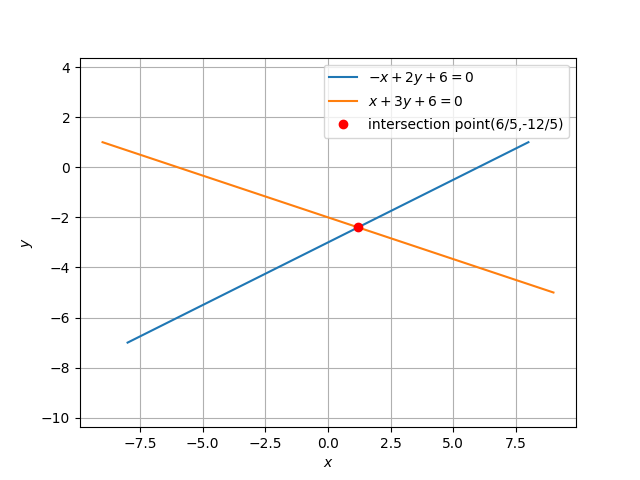
\includegraphics[width=\columnwidth]{./solutions/13/1/Figure_1.png}
\caption{plot showing intersection of lines.}
\label{eq:solutions/13/1/Fig_1}
\end{figure}

\item Prove that the following equations represent two straight lines; and also find their point of intersection and the angle between them
\begin{align}\nonumber
    x^2-5xy+4y^2+x+2y-2=0
\end{align}
\\
\solution
{Proving that given equation represents two straight lines}
The given equation is
\begin{align}\label{eq:solutions/13/2/eq:e1}
    x^2-5xy+4y^2+x+2y-2=0
\end{align}
Comparing this to the standard equation,
\begin{align}
    \vec{V} = \myvec{1 & \frac{-5}{2} \\ \frac{-5}{2} & 4}\\
    \vec{u} = \myvec{\frac{1}{2} \\ 1}\\
    f = -2
\end{align}
\begin{align}\label{eq:solutions/13/2/eq:e3}
    \implies\vec{x}^T\myvec{1 & \frac{-5}{2} \\ \frac{-5}{2} & 4}\vec{x} + 2\myvec{\frac{1}{2} & 1}\vec{x} -2 = 0
\end{align}
Equation \eqref{eq:solutions/13/2/eq:e1} represents a pair of straight lines if
\begin{align}
    \label{eq:solutions/13/2/eq:det}\mydet{\vec{V} & \vec{u}\\ \vec{u}^T & f}=0
\end{align}
\begin{align}
    \delta & = \mydet{1 & \dfrac{-5}{2} & \dfrac{1}{2} \\ \dfrac{-5}{2} & 4 & 1 \\ \dfrac{1}{2} & 1 & -2} \\ & = 0
\end{align}
Hence, proved that given equation represents two straight lines.
{Finding point of intersection between the straight lines}
\begin{align}
    \det V & = \mydet{1 & \frac{-5}{2}\\ \frac{-5}{2} & 4}\\ & = \frac{-9}{4} < 0
\end{align}
Thus, the two straight lines intersect. Let the equation of the straight lines be given as
\begin{align}
    \label{eq:solutions/13/2/eq:line1}\vec{n}_1^T\vec{x}=c_1 \\
    \label{eq:solutions/13/2/eq:line2}\vec{n}_2^T\vec{x}=c_2
\end{align}
with their slopes as $\vec{m}_1$ and $\vec{m}_2$ respectively.

Then the equation of the pair of straight lines is
\begin{align}\label{eq:solutions/13/2/eq:line1line2}
    (\vec{n}_1^T\vec{x}-c_1)(\vec{n}_2^T\vec{x}-c_2) = 0
\end{align}
Using \eqref{eq:solutions/13/2/eq:e3} and \eqref{eq:solutions/13/2/eq:line1line2},
\begin{align}
    (\vec{n}_1^T\vec{x}-c_1)(\vec{n}_2^T\vec{x}-c_2) = \vec{x}^T\myvec{1 & \frac{-5}{2} \\ \frac{-5}{2} & 4}\vec{x} + 2\myvec{\frac{1}{2} & 1}\vec{x} -2
\end{align}
Comparing both sides,
\begin{align}
    c_2\vec{n}_1+c_1\vec{n}_2 = -2\myvec{\frac{1}{2} \\ 1}\label{eq:solutions/13/2/eq:c1c2}\\
    c_1c_2 = -2
\end{align}
Slopes of the lines are roots of the equation
\begin{align}
    cm^2+2bm+a=0 \label{eq:solutions/13/2/eq:slope}\\
    \implies m_i = \frac{-b\pm \sqrt{-\mydet{\vec{V}}}}{c}\\
    \vec{n}_i = k_i\myvec{-m_i \\ 1}
\end{align}
Substituting \eqref{eq:solutions/13/2/eq:e1} in \eqref{eq:solutions/13/2/eq:slope},
\begin{align}
    4m^2-5m+1=0\\
    \implies m_i = \frac{\frac{5}{2}\pm \frac{3}{2}}{4} \\
    \implies m_1 = 1, m_2 = \frac{1}{4}
\end{align}
Therefore,
\begin{align}
    \vec{n}_1=k_1\myvec{-1 \\ 1}\\
    \vec{n}_2=k_2\myvec{\frac{-1}{4} \\ 1}
\end{align}
We know that
\begin{align}
	\label{eq:solutions/13/2/n1n2}\vec{n}_1*\vec{n}_2 = \myvec{a\\2b\\c}\\
	k_1\myvec{-1 \\ 1}*k_2\myvec{\frac{-1}{4} \\ 1} = \myvec{1 \\ -5 \\ 4}\\
	\implies k_1k_2 = 4
\end{align}
Taking $k_1 = 1$, $k_2 = 4$, we get
\begin{align}
    \vec{n}_1 = \myvec{-1 \\ 1}\nonumber\\
    \vec{n}_2 = \myvec{-1 \\ 4}\label{eq:solutions/13/2/eq:nvalues}
\end{align}
For verifying values of $\vec{n}_1$ and $\vec{n}_2$, we compute the convolution by representing $\vec{n}_1$ as Toeplitz matrix,
\begin{align}
    \vec{n}_1*\vec{n}_2=\myvec{-1 & 0 \\ 1 & -1 \\ 0 & 1}\myvec{-1 \\ 4} = \myvec{1 \\ -5 \\ 4}
\end{align}
Now, obtaining $c_1$ and $c_2$ using \eqref{eq:solutions/13/2/eq:nvalues} and \eqref{eq:solutions/13/2/eq:c1c2}
\begin{align}
    \myvec{\vec{n}_1 & \vec{n}_2}\myvec{c_2 \\ c_1} = -2\myvec{\frac{1}{2} \\ 1}\\
    \implies \myvec{-1 & -1 \\ 1 & 4}\myvec{c_2 \\ c_1} = \myvec{-1 \\ -2}
\end{align}
Row reducing the augmented matrix,
\begin{align}
    \myvec{-1 & -1 & -1 \\ 1 & 4 & -2} \xleftrightarrow{R_1 \leftarrow -R_1}\myvec{1 & 1 & 1 \\ 1 & 4 & -2}\\\xleftrightarrow{R_2\leftarrow R_2-R_1}\myvec{1 & 1 & 1 \\ 0 & 3 & -3}\\
    \xleftrightarrow{R_1\leftarrow R_1-R_2}\myvec{1 & 0 & 2 \\ 0 & 1 & -1}
\end{align}
\begin{align}
    \implies \myvec{1 & 0 \\ 0 & 1}\myvec{c_2 \\ c_1} = \myvec{2 \\ -1}\nonumber\\
    c_1 = -1\\
    c_2 = 2\label{eq:solutions/13/2/eq:cvalues}
\end{align}
Thus, equation of lines can be written as
\begin{align}
    \myvec{-1 & 1}\vec{x} = -1\\
    \myvec{-1 & 4}\vec{x} = 2
\end{align}
Augmented matrix for these set of equations is
\begin{align}
    \myvec{-1 & 1 & -1 \\ -1 & 4 & 2}\xleftrightarrow{R_1\leftarrow -R_1}\myvec{1 & -1 & 1 \\ -1 & 4 & 2}\\\xleftrightarrow{R_2\leftarrow R_2+R_1}\myvec{1 & -1 & 1 \\ 0 & 3 & 3}
    \xleftrightarrow{R_2\leftarrow \frac{R_2}{3}}\myvec{1 & -1 & 1 \\ 0 & 1 & 1}\\\xleftrightarrow{R_1\leftarrow R_1+R_2}\myvec{1 & 0 & 2 \\ 0 & 1 & 1}
\end{align}
Thus, the point of intersection is $\vec{A} = \myvec{2 \\ 1}$.
\begin{figure}[h!]
    \centering
    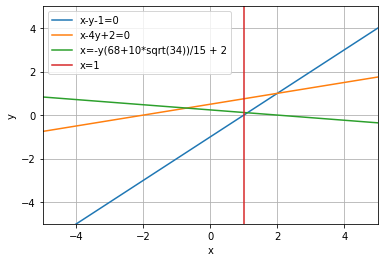
\includegraphics[width=\columnwidth]{./solutions/13/2/assignment3.png}
    \caption{Intersection of pair of original pair of straight lines and the pair of straight lines after affine transform}
    \label{eq:solutions/13/2/fig:fig1}
\end{figure}

Using \eqref{eq:solutions/13/2/eq:nvalues} and \eqref{eq:solutions/13/2/eq:cvalues} in \eqref{eq:solutions/13/2/eq:line1line2}, equation of the pair of straight lines is
\begin{align}
    (x-y-1)(x-4y+2) = 0
\end{align}

{Angle between lines}
Angle between pair of lines is,
\begin{align}\label{eq:solutions/13/2/eq:cos}
    \theta = \cos^{-1}\left(\frac{\vec{n}_1^T\vec{n}_2}{\norm{\vec{n}_1}\norm{\vec{n}_2}}\right)
\end{align}
\begin{align}
    \vec{n}_1^T\vec{n}_2 = \myvec{-1 & 1}\myvec{-1 \\ 4} = 5 \label{eq:solutions/13/2/eq:a2} 
\end{align}
\begin{align}
    \norm{\vec{n}_1}=\sqrt{(-1)^2+1^2}=\sqrt{2}\\
    \norm{\vec{n}_2}=\sqrt{(-1)^2+4^2}=\sqrt{17} \label{eq:solutions/13/2/eq:}
\end{align}
Substituting these values \eqref{eq:solutions/13/2/eq:cos}
\begin{align}
    \theta = 30.9\degree
\end{align}
Hence, angle between the given pair of straight lines is $30.9\degree$
{Affine Transformation and Eigen Value decomposition}
First, verifying if $\vec{u}^T\vec{V}^{-1}\vec{u}-f = 0$. To do this, finding $V^{-1}$ by augmenting with identity matrix and row reducing as follows :
\begin{align}
    \myvec{1 & \frac{-5}{2} & 1 & 0\\ \frac{-5}{2} & 4 & 0 & 1}\xleftrightarrow{R_2\leftarrow R_2 + \frac{5}{2}R_1}\myvec{1 & \frac{-5}{2} & 1 & 0\\ 0 & \frac{-9}{4} & \frac{5}{2} & 1}\\\xleftrightarrow{R_2\leftarrow\frac{-4}{9}R_2}\myvec{1 & \frac{-5}{2} & 1 & 0\\ 0 & 1 & \frac{-10}{9} & \frac{-4}{9}}\\\xleftrightarrow{R_1\leftarrow R_1 + \frac{5}{2}R_2}\myvec{1 & 0 & \frac{-16}{9} & \frac{-10}{9}\\ 0 & 1 & \frac{-10}{9} & \frac{-4}{9}}\\
    \implies\vec{V}^{-1} = \myvec{\frac{-16}{9} & \frac{-10}{9} \\ \frac{-10}{9} & \frac{-4}{9}}
\end{align}
\begin{align}
    u^TV^{-1}u-f & = \myvec{\frac{1}{2} & 1}\myvec{\frac{-16}{9} & \frac{-10}{9} \\ \frac{-10}{9} & \frac{-4}{9}}\myvec{\frac{1}{2} \\ 1} - (-2) \\ & = 0
\end{align}
The characteristic equation of $\vec{V}$ is given as :
\begin{align}
    \mydet{\lambda\vec{I}-\vec{V}} = \mydet{\lambda - 1 & \frac{5}{2} \\ \frac{5}{2} & \lambda - 4} = 0\\
    \implies (\lambda - 1)(\lambda - 4) - \dfrac{25}{4} = 0\\
    \label{eq:solutions/13/2/eq:characteristic}\implies 4\lambda^2-20\lambda-9 = 0
\end{align}
The roots of \eqref{eq:solutions/13/2/eq:characteristic}, i.e. the eigenvalues of $\vec{V}$ are
\begin{align}
    \lambda_1 = \dfrac{5+\sqrt{34}}{2}, \lambda_2 = \dfrac{5-\sqrt{34}}{2}\label{eq:solutions/13/2/eq:eigenval}
\end{align}
The eigen vector $\vec{p}$ is defined as, 
\begin{align}
    \vec{V}\vec{p} &= \lambda\vec{p}\\
    \implies(\lambda\vec{I}-\vec{V})\vec{p}=0
\end{align}
For $\lambda_1=\dfrac{5+\sqrt{34}}{2}$
\begin{align}
    (\lambda_1\vec{I}-\vec{V}) = \myvec{\frac{3+\sqrt{34}}{2} & \frac{5}{2} \\ \frac{5}{2} & \frac{-3 +\sqrt{34}}{2}}
\end{align}
To find $\vec{p}_1$, let's look at Augmented form of $(\lambda_1\vec{I}-\vec{V})$
\begin{align}
    \myvec{\frac{3+\sqrt{34}}{2} & \frac{5}{2} & 0 \\ \frac{5}{2} & \frac{-3 +\sqrt{34}}{2} & 0}\\\xleftrightarrow{R_1 \leftarrow \frac{2}{3+\sqrt{34}}R_1}\myvec{1 & \frac{-3+\sqrt{34}}{5} & 0 \\ \frac{5}{2} & \frac{-3 +\sqrt{34}}{2} & 0}\\\xleftrightarrow{R_2\leftarrow \frac{2}{5}R_2 - R_1}\myvec{1 & \frac{-3+\sqrt{34}}{5} & 0 \\ 0&0&0}
\end{align}
So we get
\begin{align}
    x_1 + \left(\frac{-3+\sqrt{34}}{5}\right) x_2 = 0
\end{align}
Thus, our eigenvector corresponding to $\lambda_1$
\begin{align}
    \vec{p}_1 = \myvec{\frac{3-\sqrt{34}}{5} \\ 1}
\end{align}
For $\lambda_2=\dfrac{5-\sqrt{34}}{2}$
\begin{align}
    (\lambda_2\vec{I}-\vec{V}) = \myvec{\frac{3-\sqrt{34}}{2} & \frac{5}{2} \\ \frac{5}{2} & \frac{-3 -\sqrt{34}}{2}}
\end{align}
To find $\vec{p}_2$, let's look at Augmented form of $(\lambda_2\vec{I}-\vec{V})$
\begin{align}
    \myvec{\frac{3-\sqrt{34}}{2} & \frac{5}{2} & 0 \\ \frac{5}{2} & \frac{-3 -\sqrt{34}}{2} & 0}\\\xleftrightarrow{R_1 \leftarrow \frac{2}{3-\sqrt{34}}R_1}\myvec{1 & \frac{-3-\sqrt{34}}{5} & 0 \\ \frac{5}{2} & \frac{-3 -\sqrt{34}}{2} & 0}\\\xleftrightarrow{R_2\leftarrow \frac{2}{5}R_2 - R_1}\myvec{1 & \frac{-3-\sqrt{34}}{5} & 0 \\ 0&0&0}
\end{align}
So we get
\begin{align}
    x_1 + \left(\frac{-3-\sqrt{34}}{5}\right) x_2 = 0
\end{align}
Thus, our eigenvector corresponding to $\lambda_2$
\begin{align}
    \vec{p}_2 = \myvec{\frac{3+\sqrt{34}}{5} \\ 1}
\end{align}
We know $\vec{V} = \vec{P}\vec{D}\vec{P}^{T}$, where $\vec{P}$ and the diagonal matrix $\vec{D}$ are given as:
\begin{align}
    \vec{D} & = \myvec{\lambda_1 & 0 \\ 0 & \lambda_2}\\ & = \myvec{\frac{5+\sqrt{34}}{2} & 0\\ 0 & \frac{5-\sqrt{34}}{2}}\label{eq:solutions/13/2/eq:DVal}\\
    \vec{P} & = \myvec{\vec{p}_1 & \vec{p}_2}\\&= \myvec{\frac{3-\sqrt{34}}{5} & \frac{3+\sqrt{34}}{5}\\ 1 & 1}\label{eq:solutions/13/2/eq:PVal}
\end{align}
So, the equation of the pair of straight lines is given by :
\begin{align}
    \vec{y}^T\vec{D}\vec{y} = \vec{u}^T\vec{V}^{-1}\vec{u}-f\qquad\text{$\mydet{\vec{V}}\neq0$}\\
    \vec{y}^T\myvec{\dfrac{5+\sqrt{34}}{2} & 0\\ 0 & \dfrac{5-\sqrt{34}}{2}}\vec{y} =0\\
    \implies \myvec{y_1 & y_2}\myvec{\dfrac{5+\sqrt{34}}{2} & 0\\ 0 & \dfrac{5-\sqrt{34}}{2}}\myvec{y_1 \\ y_2} = 0\\
    \implies (5+\sqrt{34})y_1^2 + (5-\sqrt{34})y_2^2 = 0
\end{align}
So we get the equation of the pair of straight lines, as we can see this passes through the origin $(0,0)$. The corresponding image is shown in Fig. \ref{eq:solutions/13/2/fig:fig2}
\begin{align}
    \vec{c} = -\vec{V}^{-1}\vec{u}\qquad\text{$\mydet{\vec{V}}\neq0$}\\
    \implies \vec{c} = -\myvec{\frac{-16}{9} & \frac{-10}{9} \\ \frac{-10}{9} & \frac{-4}{9}}\myvec{\frac{1}{2} \\ 1} = \myvec{2 \\ 1}\\
    \intertext{And,}
    \vec{P}^T = \myvec{\frac{3-\sqrt{34}}{5} & 1\\ \frac{3+\sqrt{34}}{5} & 1}
    \intertext{Using affine transformation, we can express the equation as}
    \vec{x} = \vec{P}\vec{y} + \vec{c}\\
    \implies \vec{x} = \myvec{\frac{3-\sqrt{34}}{5} & \frac{3+\sqrt{34}}{5}\\1 & 1}\vec{y} + \myvec{2 \\ 1}
\end{align}
The corresponding image is shown in Fig. \ref{eq:solutions/13/2/fig:fig1}
\begin{figure}[h!]
    \centering
    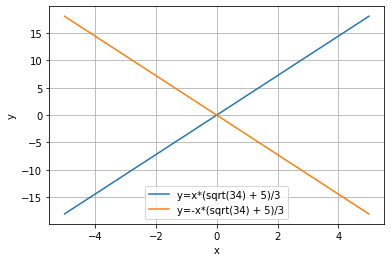
\includegraphics[width=\columnwidth]{./solutions/13/2/assignment3.1.png}
    \caption{Pair of straight lines passing through origin after eigenvalue decomposition}
    \label{eq:solutions/13/2/fig:fig2}
\end{figure}

\item Prove that the following equations represent two straight lines.Also find their point of intersection and the angle between them
\begin{align}
 3y^2-8xy-3x^2-29x+3y-18=0   
\label{eq:solutions/13/3/1}
\end{align}
\solution
\mydet{\vec{V}&\vec{u}\\\vec{u}^T&f} of \eqref{eq:solutions/13/3/1} becomes
\begin{align}
    \mydet{-3&-4&-\frac{29}{2}\\-4&3&\frac{3}{2}\\-\frac{29}{2}&\frac{3}{2}&-18}\label{eq:solutions/13/3/2}
\end{align}
Expanding equation \eqref{eq:solutions/13/3/2}, we get zero.\\
Hence given equation represents a pair of straight lines.
Slopes of the individual lines are roots of equation 
\begin{align}
    cm^2+2bm+a=0\\
    \implies 3m^2-8m-3=0\\
    \text{Solving, }m=3,-\frac{1}{3}
\end{align}
The normal vectors of the lines then become
\begin{align}
    \vec{n_1}=\myvec{\frac{1}{3}\\1}\\
    \vec{n_2}=\myvec{-3\\1}
\end{align}
Equations of the lines can therefore be written as
\begin{align}
  \myvec{\frac{1}{3}&1}\vec{x}=c\\
 \implies \myvec{1&3}\vec{x}=c_1 ,\\
   \myvec{-3&1}\vec{x}=c_2\\
  \implies \left[\myvec{1&3}\vec{x}-c_1\right]\left[\myvec{-3&1}\vec{x}-c_2\right]
\end{align}
represents the equation specified in \eqref{eq:solutions/13/3/1}\\
Comparing the equations, we have
\begin{align}
    \myvec{1&-3\\3&1}\myvec{c_2\\c_1}=\myvec{29\\-3}\\
 \end{align}
 Row reducing the augmented matrix
 \begin{align}
    \myvec{1&-3&29\\3&1&-3}\xleftrightarrow[]{R_2\leftarrow R_2-3\times R_1}
    \myvec{1&-3&29\\0&10&-90}\\
    \xleftrightarrow[]{R_2\leftarrow R_2\times \frac{1}{10}}
    \myvec{1&-3&29\\0&1&-9}\\
    \xleftrightarrow[]{R_1\leftarrow R_1+3\times R_2}
    \myvec{1&0&2\\0&1&-9}\\
    \implies c_2=2 \text{ and }c_1=-9
\end{align}
The individual line equations therefore become
\begin{align}
    \myvec{1&3}\vec{x}=-9\label{eq:solutions/13/3/3} ,\\\myvec{-3&1}\vec{x}=2\label{eq:solutions/13/3/4}
\end{align}
Note that the convolution of the normal vectors, should satisfy the below condition
\begin{align}
    \myvec{1\\3}*\myvec{-3\\1}=\myvec{a\\2b\\c}\label{eq:solutions/13/3/5}
\end{align}
The LHS part of \eqref{eq:solutions/13/3/5} can be rewritten using toeplitz matrix as
\begin{align}
    \myvec{1&0\\3&1\\0&3}\myvec{-3\\1}=\myvec{-3\\-8\\3}=\myvec{a\\2b\\c}
\end{align}

The augmented matrix for the set of equations represented in \eqref{eq:solutions/13/3/3}, \eqref{eq:solutions/13/3/4} is
\begin{align}
\myvec{1&3&-9\\-3&1&2}
\end{align}
Row reducing the matrix
\begin{align}
 \myvec{1&3&-9\\-3&1&2}\xleftrightarrow[]{R_2\leftarrow R_2+3\times R_1}\myvec{1&3&-9\\0&10&-25}\\
 \xleftrightarrow[]{R_1\leftarrow R_1-\frac{3}{10}\times R_2}\myvec{1&0&-\frac{3}{2}\\0&10&-25}\\
 \xleftrightarrow[]{R_2\leftarrow \frac{R_2}{10}}\myvec{1&0&-\frac{3}{2}\\0&1&-\frac{5}{2}}\\
\text{Hence, the intersection point is}
\myvec{-\frac{3}{2}\\-\frac{5}{2}}
\end{align}
\begin{figure}[!ht]
\centering
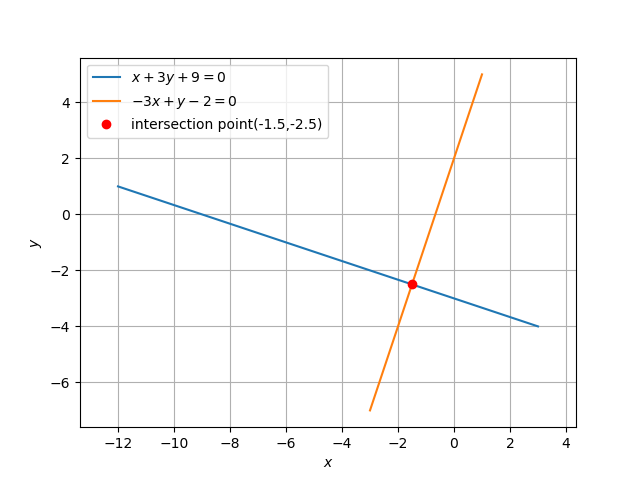
\includegraphics[width=\columnwidth]{./solutions/13/3/hw4plot.png}
\caption{plot showing intersection of lines}
\label{eq:solutions/13/3/Fig:solutions/13/3/}
\end{figure}
Angle between two lines $\theta$ can be given by
\begin{align}
\cos \theta = \frac{\vec{n_1}^T\vec{n_2}}{\norm{\vec{n_1}}\norm{\vec{n_2}}}
\end{align}
%From \eqref{eq:solutions/13/3/3}, \eqref{eq:solutions/13/3/4},
\begin{align}
\cos \theta=\frac{\myvec{1&3}\myvec{-3\\1}}{\sqrt{(3)^2 +1} \times \sqrt{(-3)^2 +1}}=0\\
\implies \theta = 90\degree
\end{align}


\item Prove that the following equations represents two straight lines also find their point of intersection and angle between them.
\begin{align}
y^2+xy-2x^2-5x-y-2=0
\end{align}
%
\solution
\begin{align}
\vec{V}=\myvec{a&b\\b&c}=\myvec{-2&\frac{1}{2}\\\frac{1}{2}&1}\\
\vec{u}=\myvec{d\\e}=\myvec{\frac{-5}{2}\\\frac{-1}{2}}\\
f=-2
\end{align}
\begin{align}
\mydet{
-2&\frac{1}{2}&\frac{-5}{2}\\
\frac{1}{2}&1&\frac{-1}{2}\\
\frac{-5}{2}&\frac{-1}{2}&-2}
\xleftrightarrow[R_1\rightarrow R_1+R_3]{R_1\rightarrow R_1-R_2}
\mydet{
0&0&0\\
\frac{1}{2}&1&\frac{-1}{2}\\
\frac{-5}{2}&\frac{-1}{2}&-2}=0
\end{align}
Hence it represents the pair of straight lines.
Now two intersecting lines are obtained when
\begin{align}
\mydet{V} < 0 
\implies \mydet{-2&\frac{1}{2}\\\frac{1}{2}&1}
=\frac{-9}{4} < 0
\end{align}
Let the pair of straight of lines be given by
\begin{align}
\vec{n_1}^T\vec{x}=c_1\\
\vec{n_2}^T\vec{x}=c_2
\end{align}
The slopes of the lines are given by the roots of the polynomial 
\begin{align}
cm^2+2bm+a=0 \\
m_1,m_2 = \frac{-\frac{1}{2}\pm\sqrt{\frac{9}{4}}}{1}\\
m_1= 1 , m_2 =-2\\
\implies\vec{n_1}=\myvec{-1\\1} and \vec{n_2}=\myvec{2\\1}
\end{align}
\begin{align}
(\vec{n_1}^T\vec{x}-c_1)(\vec{n_2}^T\vec{x}-c_2) =
\vec{x}^T\vec{V}\vec{x}+2\vec{u}^T\vec{x}+f 
\end{align}
\begin{align}
c_2\vec{n_1}+c_1\vec{n_2} =-2\vec{u}
 \end{align}
 \begin{align}
 c_2\myvec{-1\\1}+c_1\myvec{2\\1} =-2\myvec{\frac{-5}{2}\frac{-1}{2}}
 \end{align}
 \begin{align}
 \myvec{1&1\\2&-1}\myvec{c_1\\c_2}=\myvec{1\\5}
 \end{align}
 Using row reduction we get
 \begin{align}
\myvec{1&1&1\\2&-1&5}\\
\xleftrightarrow[R_2\leftarrow R_2/-3]{R_2\leftarrow R_2-2R_1}
\myvec{1&1&1\\0&1&-1}\\\xleftrightarrow[]{R_1\leftarrow R_1-R_2}
\myvec{1&0&2\\0&1&-1}
\end{align}
\begin{align}
C  =\myvec{2\\-1}
\end{align}
 The convolution of the normal vectors, should satisfy the below condition
 \begin{align}
    \myvec{-1\\1}*\myvec{2\\1}=\myvec{a\\2b\\c}
\end{align}
The LHS part of equation(2.0.20) can be rewritten using toeplitz matrix as
\begin{align}
    \myvec{-1&0\\1&-1\\0&1}\myvec{2\\1}=\myvec{-2\\1\\1}=\myvec{a\\2b\\c}
\end{align}
Therefore the equation of lines is given by 
\begin{align}
\myvec{-1&1}\vec{x}=2\\
\myvec{2&1}\vec{x}=-1
\end{align}
consider the augmented matrix
\begin{align}
\myvec{-1&1&2\\2&1&-1}\\
\xleftrightarrow[R_2\leftarrow R_2-2R_1]{R_1\leftarrow -R_1}
\myvec{1&2&1\\0&1&1}\\\xleftrightarrow[R_1\leftarrow R_1+R_2]{R_1\leftarrow R_1/3}
\myvec{1&0&-1\\0&1&1}
\end{align}
Therefore point of intersection is $\vec{A}=\myvec{-1\\1}.$
\\
Angle between two lines $\theta$ can be given by
\begin{align}
\cos\theta =\frac{\vec{n_1}^T\vec{n_2}}{\norm{\vec{n_1}}\norm{\vec{n_2}}}\\
 \cos\theta=\frac{\myvec{-1&1}\myvec{2\\1}}{\sqrt{\left(1\right)^2 +1} \times \sqrt{(2)^2 +1}}
\end{align}
\begin{align}
\theta = \cos^{-1}(\frac{-1}{\sqrt{10}})\implies \theta = tan^{-1}3
\end{align}
\begin{figure}[!ht]
\centering
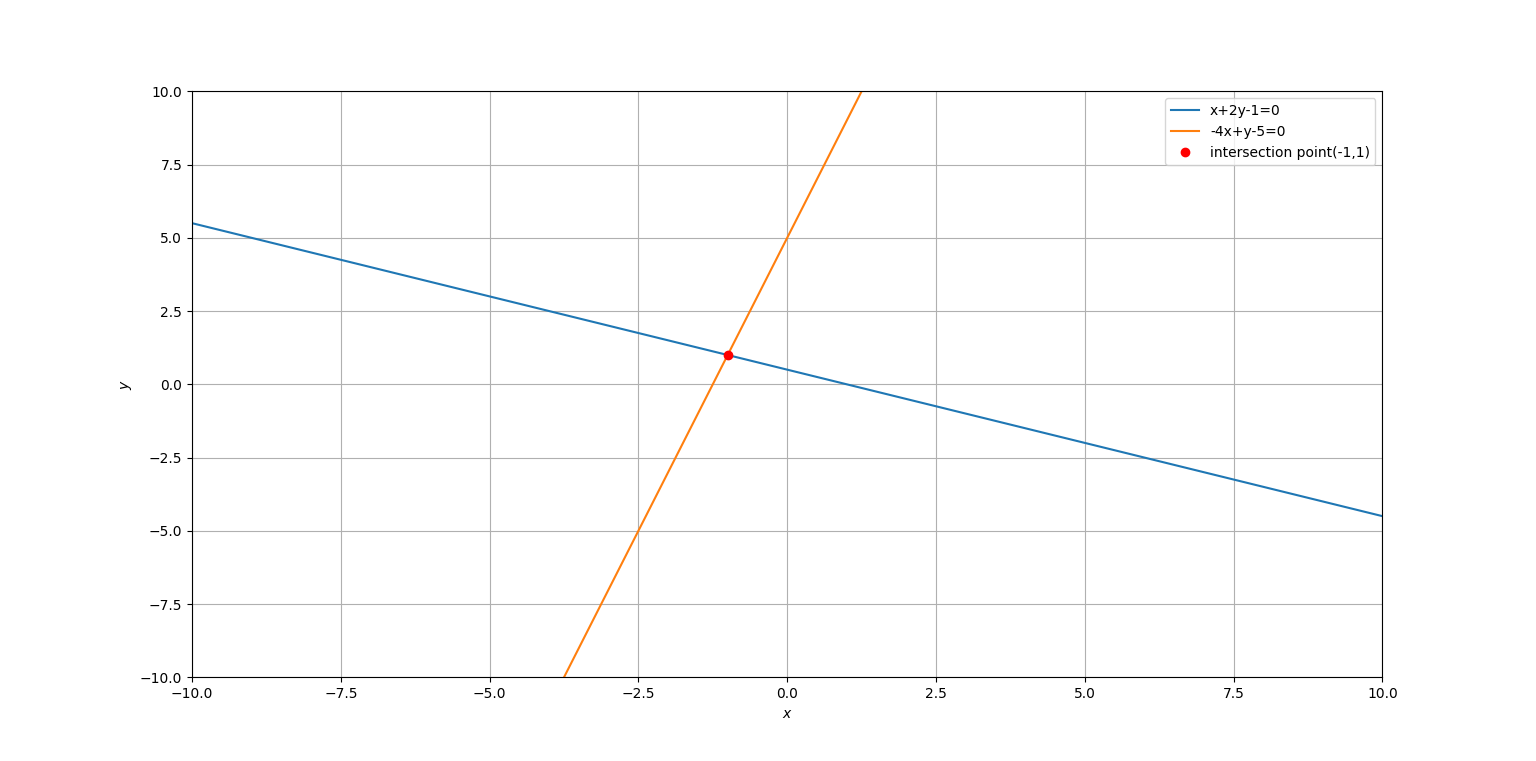
\includegraphics[width=\columnwidth]{./solutions/13/4/Figure_2.png}
\caption{plot showing intersection of lines}
\label{Fig:solutions/13/4}
\end{figure}

\item Prove that the equation
\begin{align} 
    x^{2}+6xy+9y^{2}+4x+12y-5=0 \label{eq:solutions/13/5/eq:0}
\end{align}
represents two parallel lines.

\solution
The given equation \eqref{eq:solutions/13/5/eq:0} can be written as
\begin{align}
\vec{x}^T\myvec{1 & 3 \\ 3 & 9}\vec{x} +2\myvec{2 &6}\vec{x}-5=0\label{eq:solutions/13/5/eq:1}\\
\vec{V} = \myvec{1 & 3 \\ 3 & 9} \quad \vec{u} = \myvec{2 \\ 6} \quad f= -5 \label{eq:solutions/13/5/eq:2}
\end{align}
Equation \eqref{eq:solutions/13/5/eq:0} represents pair of straight line as,
\begin{align}
D = \mydet{1&3&2\\3&9&6\\2&6&-5} = 0
\end{align}
Vector form of straight lines,
\begin{align}
\vec{n_1}^T\vec{x}= \vec{c_1}\\
\vec{n_2}^T\vec{x} = \vec{c_2}
\end{align}
Equating their product with \eqref{eq:solutions/13/5/eq:1}
\begin{align}
(\vec{n_1}^T\vec{x} -\vec{c_1})(\vec{n_2}^T\vec{x} - \vec{c_2})= \vec{x}^T\myvec{1 & 3 \\ 3 & 9}\vec{x} +2\myvec{2 &6}\vec{x}-5
\end{align}
\begin{align}
\vec{n_1}*\vec{n_2}=\myvec{1\\6\\9}\label{eq:solutions/13/5/eq:3}\\
c_2\vec{n_1}+c_1\vec{n_2} = -2\myvec{2\\6}\\
c_1c_2 = -5
\end{align}
The slopes of the lines can be given by roots of the equation,
\begin{align} 
cm^2+2bm+a=0 \label{eq:solutions/13/5/eq:4}\\
m_i = \frac{-b\pm \sqrt{-\mydet{\vec{V}}}}{c}\label{eq:solutions/13/5/eq:5}\\
\vec{n_i}=k_i\myvec{-m_i\\1}\label{eq:solutions/13/5/eq:6}
\end{align}
From \eqref{eq:solutions/13/5/eq:1} equation \eqref{eq:solutions/13/5/eq:4} becomes
\begin{align}
9m^2+6m+1=0
\end{align}
Using \eqref{eq:solutions/13/5/eq:2},
\begin{align}
\mydet{\vec{V}} = \mydet{1 & 3\\ 3 & 9} = 0
\end{align}
Substituting the values in \eqref{eq:solutions/13/5/eq:5},
\begin{align}
m_i = \frac{-3\pm 0}{9}\\
m_1= m_2 = \frac{-1}{3} \label{eq:solutions/13/5/eq:7}
\end{align}
Substituting values in \eqref{eq:solutions/13/5/eq:6}
\begin{align}
\vec{n_1}=k_1\myvec{\frac{1}{3}\\1}\\
\vec{n_2}=k_2\myvec{\frac{1}{3}\\1}
\end{align}
Using the above values in \eqref{eq:solutions/13/5/eq:3},
\begin{align}
k_1k_2 = 9
\end{align}
Taking $k_1=3$ and $k_2 = 3$ we get
\begin{align}
\vec{n_1}=\myvec{1\\3}\\
\vec{n_2}=\myvec{1\\3}
\end{align}
Verifying $\vec{n_1}$ and $\vec{n_2}$ by computing the convolution by representing $\vec{n_1}$ as Toeplitz matrix,
\begin{align}
\vec{n_1}*\vec{n_2}=\myvec{1&0\\3&1\\0&3}\myvec{1\\3}=\myvec{1\\6\\9}
\end{align}
Finding the Angle between the lines,
\begin{align}
\theta = \cos^{-1}\brak{\frac{\vec{n_1}^T\vec{n_2}}{\norm{\vec{n_1}}\norm{\vec{n_2}}}}\label{eq:solutions/13/5/eq:8}\\
\vec{n_1}^T\vec{n_2} = \myvec{1&3}\myvec{1\\3} = 10 \label{eq:solutions/13/5/eq:9}\\
\norm{\vec{n_1}} = \sqrt{10}\quad \norm{\vec{n_2}}=\sqrt{10} \label{eq:solutions/13/5/eq:10}
\end{align}
Substituting \eqref{eq:solutions/13/5/eq:9} and \eqref{eq:solutions/13/5/eq:10} in \eqref{eq:solutions/13/5/eq:8} we get,
\begin{align}
\theta = \cos^{-1}(1)\\
\theta = 0^{\circ}\label{eq:solutions/13/5/eq:11}
\end{align}
From \eqref{eq:solutions/13/5/eq:7} and \eqref{eq:solutions/13/5/eq:11} shows the given equation \eqref{eq:solutions/13/5/eq:0} represents two parallel lines. Hence proved.
\begin{figure}[!ht]
\centering
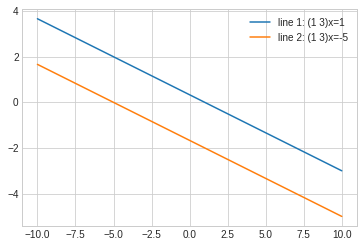
\includegraphics[width=\columnwidth]{./solutions/13/5/Straight_lines.png}
\caption{Pair of straight lines plot generated using python}
\label{eq:solutions/13/5/fig:plot}
\end{figure}

\item 
%
\solution
Find the value of k such that 
\begin{align}
	6x^2 + 11xy - 10y^2 + x + 31y + k =0 \label{eq:solutions/13/6/eq:eq5}
\end{align}

represent pairs of straight lines.

From \eqref{eq:solutions/13/6/eq:eq5} we get,
\begin{align}
	\vec{V} &= \myvec{6 & \frac{11}{2} \\ \frac{11}{2} & -10}\\
	\vec{u} &= \myvec{\frac{1}{2}\\ \frac{31}{2}}\\
	f &= k
\end{align}
Compute the slopes of lines given by the roots of the polynomial $-10m^2 + 11m + 6$
\begin{align}
   i.e., m_i &= \frac{-b \pm \sqrt{- \mydet{\vec{V}}}}{c} \label{eq:solutions/13/6/eq:eq2} \\
   \implies m &= \frac{\frac{-11}{2} \pm \frac{19}{2}}{-10} \\ 
   \implies m_1 &= \frac{-2}{5}, m_2 = \frac{3}{2} 
\end{align} 
Let the pair of straight lines be given by 
\begin{align}
	\vec{n}_1^T\vec{x} = c_1 \label{eq:solutions/13/6/eq:n_1}\\
	\vec{n}_2^T\vec{x} = c_2 \label{eq:solutions/13/6/eq:n_2}
\end{align}
Here,
\begin{align}
	\vec{n}_1 &= k_1\myvec{-m_1\\1} = k_1 \myvec{ \frac{2}{5} \\ 1}  \label{eq:solutions/13/6/eq:n1val}\\
	\vec{n}_2 &= k_2\myvec{-m_2\\1} = k_2 \myvec{\frac{-3}{2} \\ 1} \label{eq:solutions/13/6/eq:n2val}
\end{align}
We know that, 
\begin{align}
	\vec{n}_1 * \vec{n}_2 = \myvec{a\\2b\\c} \label{eq:solutions/13/6/eq:n1n2}
\end{align}
Substituting \eqref{eq:solutions/13/6/eq:n1val} and \eqref{eq:solutions/13/6/eq:n2val} in the above equation, we get
\begin{align}
	k_1 \myvec{ \frac{2}{5} \\ 1} * k_2 \myvec{\frac{-3}{2} \\ 1} &= \myvec{6\\ 11\\ -10}\\
	\implies k_1k_2 &= -10
\end{align} 
By inspection, we get the values, $k_1 = 5, k_2 = -2$. Substituting the values of $k_1$ and $k_2$ in \eqref{eq:solutions/13/6/eq:n1val} and \eqref{eq:solutions/13/6/eq:n2val} respectively, we get
\begin{align}
	\vec{n}_1 &= \myvec{2 \\ 5} \label{eq:solutions/13/6/eq:n1}\\
	\vec{n}_2 &= \myvec{3 \\ -2} \label{eq:solutions/13/6/eq:n2}
\end{align}
Using Teoplitz matrix representation, the convolution of $\vec{n}_1$ with $\vec{n}_2$, is as follows:
\begin{align}
	\myvec{2 & 0 & 5\\ 5 & 2 & 0\\ 0 & 5 & 2}\myvec{3\\-2\\0} = \myvec{6 \\11 \\ -10} = \myvec{a \\ 2b \\ c}
\end{align}
Hence, $\vec{n}_1$ and $\vec{n}_2$ satisfies \eqref{eq:solutions/13/6/eq:n1n2}.
We have,
\begin{align}
	c_2\vec{n}_1 + c_1\vec{n}_2 &= -2\vec{u} \label{eq:solutions/13/6/eq:cneq}
\end{align}
Substituting \eqref{eq:solutions/13/6/eq:n1}, \eqref{eq:solutions/13/6/eq:n2} in \eqref{eq:solutions/13/6/eq:cneq}, we get
\begin{align}
 \myvec{2 & 3\\ 5 & -2}\myvec{c_2 \\ c_1} &= -2\myvec{\frac{1}{2} \\ \frac{31}{2}}
\end{align}
Solving for $c_1$ and $c_2$, the augmented matrix is,
\begin{align}
	\myvec{2 & 3 & -1\\ 5 & -2 & -31} &\xleftrightarrow[R_2 \leftarrow R_2 - 5R_1]{R_1 \leftarrow \frac{R_1}{2}} \myvec{1 & \frac{3}{2}  & \frac{-1}{2} \\ 0 & \frac{-19}{2} & \frac{-57}{2}} \\
	&\xleftrightarrow[R_1 \leftarrow R_1 - \frac{3}{2}R_2]{R_2 \leftarrow \frac{R_2}{-19/2}} \myvec{1 & 0 & -5\\0 & 1 & 3}
\end{align}
Hence we obtain,
\begin{align}
	c_1 = 3, c_2 = -5
\end{align}
We know that,
\begin{align}
	f = k = c_1c_2\\
	\implies \boxed{k = -15}
\end{align}
Hence the solution. Using \eqref{eq:solutions/13/6/eq:n_1} and \eqref{eq:solutions/13/6/eq:n_2}, the equation of pair of straight lines is given by,
\begin{align}
\myvec{2 & 5}\vec{x} &= 3\\
\myvec{3 & -2}\vec{x} &= -5
\end{align}
See Fig. \ref{fig:solutions/13/6/}


\begin{figure}[!ht] 
	\centering
	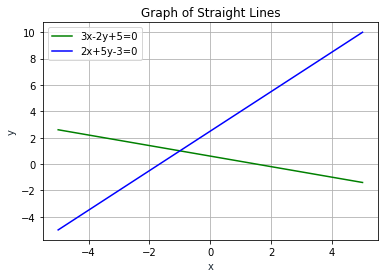
\includegraphics[width=\columnwidth]{./solutions/13/6/a6_graph.png}
	\caption{Plot of two straight lines.}
\label{fig:solutions/13/6/}
\end{figure}

%
\item Find the value of k so that following equation may represent pairs of straight lines,
\begin{align}
12x^2-10xy+2y^2+11x-5y+k=0
\label{eq:solutions/13/7/1}
\end{align}
%
\solution
The general equation of second degree is given by,
\begin{align}
ax^2 + 2bxy + cy^2 + 2dx +2ey +f = 0
\label{eq:solutions/13/7/2}
\end{align}
In vector from the equation \eqref{eq:solutions/13/7/2} can be expressed as,
\begin{align}
\vec{x}^T\vec{V}\vec{x} + 2\vec{u}^T\vec{x} + f = 0 
\label{eq:solutions/13/7/line_vec}
\end{align}
where,
\begin{align}
\vec{V} = \vec{V}^T = \myvec{a&b\\b&c}
\label{eq:solutions/13/7/3}
\end{align}
\begin{align}
\vec{u} = \myvec{d\\e}
\label{eq:solutions/13/7/4}
\end{align}
Now, comparing \eqref{eq:solutions/13/7/2} to \eqref{eq:solutions/13/7/1} we get, a =12, b=-5, c = 2, d = $\frac{11}{2}$,e = -$\frac{5}{2}$, f = k.  
Hence, substituting these values in \eqref{eq:solutions/13/7/3} and \eqref{eq:solutions/13/7/4} we get,
\begin{align}
\vec{V} = \myvec{12 & -5 \\ -5 & 2}
\end{align}
\begin{align}
\vec{u} = \myvec{\frac{11}{2} \\ -\frac{5}{2}}
\end{align}
\eqref{eq:solutions/13/7/1} represents pair of straight lines if,
\begin{align}
\mydet{\vec{V}&\vec{u}\\\vec{u}^T&f} = 0
\end{align}
\begin{align}
\mydet{12&-5&\frac{11}{2}\\-5&2&-\frac{5}{2}\\\frac{11}{2}&-\frac{5}{2}&k} = 0
\end{align}
\begin{align}
\implies k =2
\label{eq:solutions/13/7/5}
\end{align}
Lines Intercept if
\begin{align}
    |\vec{V}|<0\\
    |\vec{V}|=-1<0
\end{align}
Hence Line intercept.\\
Let $(\alpha,\beta)$ be their point of intersection, then
\begin{equation}\label{eq:solutions/13/7/eq6}
	\myvec{ a & b\\ b & c}\myvec{\alpha \\ \beta} = \myvec{-d \\ -e}
\end{equation}
Substituting in \eqref{eq:solutions/13/7/eq6}
\begin{align}
	\label{eq:solutions/13/7/eq11}\myvec{ 12 & -5\\-5 & 2}\myvec{\alpha \\ \beta} = \myvec{-\frac{11}{2} \\ \frac{5}{2}} \\
	\label{eq:solutions/13/7/eq12}\implies \myvec{\alpha \\ \beta} = \myvec{-\frac{3}{2} \\ -\frac{5}{2}}
\end{align}
Spectral Decomposition  of $\vec{V}$ is given as
\begin{equation}
\vec{V} = \vec{P}\vec{D}\vec{P}^T
\end{equation}
\begin{align}
	\label{eq:solutions/13/7/eq7}\vec{V} &= \myvec{ 12 & -5\\ -5 & 2}\\
	\label{eq:solutions/13/7/eq8}\vec{P} &= \myvec{-1-\sqrt{2} & -1 + \sqrt{2}\\ 1 & 1}\\
	\label{eq:solutions/13/7/eq9}\vec{D} &= \myvec{7 + 5\sqrt{2} & 0\\ 0 & 7 - 5\sqrt{2}}
\end{align}
Using Spectral decomposition concept and substution
\begin{align}
u_1(x-\alpha) + u_2(y-\beta) &= \pm \sqrt{-\frac{\lambda_2}{\lambda_1}}(v_1(x-\alpha) + v_2(y-\beta))\label{eq:solutions/13/7/eq10}
\end{align}
Substituting \eqref{eq:solutions/13/7/eq12}, \eqref{eq:solutions/13/7/eq8} and \eqref{eq:solutions/13/7/eq9} in \eqref{eq:solutions/13/7/eq10}
\begin{multline}\label{eq:solutions/13/7/eq13}
	\brak{-1-\sqrt{2}}\brak{x- \frac{-3}{2}} + \brak{y-\frac{-5}{2}} \\= \pm \sqrt{-\frac{7 +5\sqrt{2}} {7-5\sqrt{2}}}\brak{\brak{-1+\sqrt{2}}\brak{x- \frac{-3}{2}} + \brak{y-\frac{-5}{2}}}
\end{multline}
Simplifying \eqref{eq:solutions/13/7/eq13},
\begin{align}
	\label{eq:solutions/13/7/eq22}-6x + 2y - 4 = 0 \text{ and } -2x + y -\frac{1}{2} = 0\\
	\implies \brak{-6x + 2y - 4}\brak{-2x + y -\frac{1}{2}} = 0
\end{align}
Thus the equation of lines are
\begin{align}
\myvec{-6&2}\vec{x} = 4\\ 
\myvec{-2&1}\vec{x} = \frac{1}{2}
\end{align}
Hence, Plot is shown below 
\begin{figure}[ht!]
\centering
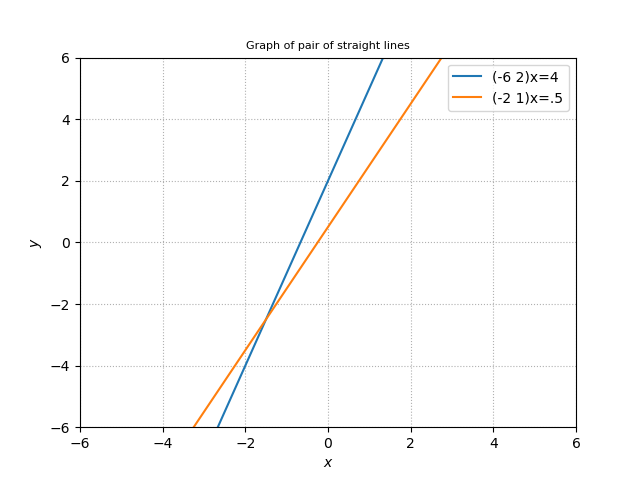
\includegraphics[width=\columnwidth]{./solutions/13/7/Figure.png}
\caption{Pair of lines}
\end{figure}

\item Find the value of k so that the following equation may represent pair of straight lines: 
\begin{align}
    12x^2+kxy+2y^2+11x-5y+2=0\label{eq:solutions/13/8/1.1}
\end{align}
\solution
\begin{align}
    \vec{V}=\vec{V}^T=\myvec{a & b \\ b & c}=\myvec{12 & \frac{k}{2} \\ \frac{k}{2} & 2}\label{eq:solutions/13/8/2.3}\\
    \vec{u}=\myvec{d \\ e}=\myvec{\frac{11}{2} \\ -\frac{5}{2}}\label{eq:solutions/13/8/2.4}
\end{align}

The equation \eqref{eq:solutions/13/8/1.1} represents pair of straight lines if
\begin{align}
    &\mydet{\vec{V} & \vec{u} \\ \vec{u}^T & f}=0\\
    \implies&\mydet{12 & \frac{k}{2} & \frac{11}{2} \\ \frac{k}{2} & 2 & -\frac{5}{2} \\ \frac{11}{2} & -\frac{5}{2} & 2}=0\label{eq:solutions/13/8/2.6}\\
    \implies&\mydet{24 & k & 11 \\ k & 4 & -5 \\ 11 & -5 & 4}=0\\
    \implies&24\mydet{ 4 & -5 \\ -5 & 4}-k\mydet{ k & -5 \\ 11 & 4}+11\mydet{ k & 4 \\ 11 & -5}=0
\end{align}
\begin{align}
    \implies2k^2+55k+350=0\\
    \implies(10+k)(2k+35)=0\\
    \implies k=-10\nonumber\\
    k=-\frac{35}{2}
\end{align}
Therefore, for $k=-10$ and $k=-\frac{35}{2}$ the given equation represents pair of straight lines.\\
Now Lets find equation of lines for $k=-10$.
\noindent
Substitute $k=-10$ in \eqref{eq:solutions/13/8/1.1}. We get equation of pair of straight lines as:
\begin{align}
    12x^2-10xy+2y^2+11x-5y+2=0
\end{align}
%Comparing above equation with \eqref{eq:solutions/13/8/2.1}, we will get $a=12$, $b=-5$, $c=2$, $d=\frac{11}{2}$, $e=-\frac{5}{2}$, $f=2$.\\
From \eqref{eq:solutions/13/8/1.1}, \eqref{eq:solutions/13/8/2.3}, \eqref{eq:solutions/13/8/2.4} we get
\begin{align}
    \vec{V}=\vec{V}^T=\myvec{12 & -5 \\ -5 & 2}\label{eq:solutions/13/8/2.17}\\
    \vec{u}=\myvec{\frac{11}{2} \\ -\frac{5}{2}}\label{eq:solutions/13/8/2.18}
\end{align}
\noindent
If $\mydet{\vec{V}}<0$ then two lines will intersect.
\begin{align}
    \mydet{\vec{V}}&=\mydet{12 & -5 \\ -5 & 2}\\
    \implies\mydet{\vec{V}}&=-1\\
    \implies\mydet{\vec{V}}&<0
\end{align}
\noindent
Therefore the lines will intersect.\\
The equation of two lines is given by
\begin{align}
    \vec{n_1}^T\vec{x}=c_1\label{eq:solutions/13/8/1.12}\\
    \vec{n_2}^T\vec{x}=c_2\label{eq:solutions/13/8/1.13}
\end{align}
Equating their product with \eqref{eq:solutions/13/8/1.1}
\begin{multline}
    (\vec{n_1}^T\vec{x}-c_1)(\vec{n_2}^T\vec{x}-c_2)\\=\vec{x}^T\vec{V}\vec{x}+2\vec{u}^T\vec{x}+f=0
\end{multline}
\begin{align}
    \implies\vec{n_1}*\vec{n_2}&=\myvec{a \\ 2b \\c}=\myvec{12\\-10\\2}\label{eq:solutions/13/8/conv}
\end{align}
\begin{align}
    c_2\vec{n_1}+c_1\vec{n_2}&=-2\vec{u}=-2\myvec{\frac{11}{2} \\ -\frac{5}{2}}\label{eq:solutions/13/8/1.16}\\
    c_1c_2&=f=2
\end{align}
The slopes of the lines are given by roots of equation
\begin{align}
    cm^2+2bm+a=0\label{eq:solutions/13/8/poly}\\
    \implies 2m^2-10m+12=0\\
    m_i=\frac{-b\pm{\sqrt{-\mydet{\vec{V}}}}}{c}\\
    \implies m_i=\frac{5\pm{\sqrt{1}}}{2}\\
    \implies m_1=3\\
     m_2=2
\end{align}
The normal vector for two lines is given by
\begin{align}
    \vec{n_i}=k_i\myvec{-m_i\\1}\label{eq:solutions/13/8/normvec}\\
    \implies\vec{n_1}=k_1\myvec{-3\\1}\label{eq:solutions/13/8/n1}\\
    \vec{n_2}=k_2\myvec{-2\\1}\label{eq:solutions/13/8/n2}
\end{align}
Substituting \eqref{eq:solutions/13/8/n1},\eqref{eq:solutions/13/8/n2} in \eqref{eq:solutions/13/8/conv}. we get
\begin{align}
    k_1k_2=2
\end{align}
The possible combinations of ($k_1$,$k_2$) are (1,2), (2,1), (-1,-2) and (-2,-1).\\
lets assume $k_1=1$,$k_2=2$ we get
\begin{align}
    \implies\vec{n_1}=\myvec{-3\\1}\label{soln1}\\
    \vec{n_2}=\myvec{-4\\2}\label{soln2}
\end{align}
We verify obtained $\vec{n_1}$,$\vec{n_2}$ using Toeplitz matrix
\begin{align}
    \vec{n_1}*\vec{n_2}=\myvec{-3 & 0\\1 & -3\\0 & 1}\myvec{-4 \\ 2}=\myvec{12\\-10\\2}\label{eq:solutions/13/8/comp1}\\
    \implies \vec{n_1}*\vec{n_2}=\myvec{12\\-10\\2}=\myvec{a\\2b\\c}
\end{align}
Therefore the obtained $\vec{n_1}$,$\vec{n_2}$ are correct.\\
Substitute \eqref{soln1}, \eqref{soln2} in \eqref{eq:solutions/13/8/1.16}
and calculate for $c_1$ and $c_2$

\begin{align}
    c_2\myvec{-3\\1}+c_1\myvec{-4\\2}=\myvec{ -11\\ -5}
\end{align}
Solve using row reduction technique.
\begin{align}
    \implies\myvec{-4 & -3 & -11\\2 & 1 & -5}\\
    \xleftrightarrow[]{R_2\leftarrow 2R_2+R_1}\myvec{-4 & -3 & -11\\0 & -1 & -21}\\
    \xleftrightarrow[]{R_1\leftarrow R_1-3R_2}\myvec{-4 & 0 & 52\\0 & -1 & -21}\\
    \implies\myvec{1 & 0 & -13\\0 & 1 & 21}\\
    \implies c_1=-13\label{c1}\\
    c_2=21\label{c2}
\end{align}

Substituting \eqref{soln1},\eqref{soln2},\eqref{c1},\eqref{c2} in \eqref{eq:solutions/13/8/1.12} and \eqref{eq:solutions/13/8/1.13}. We get equation of two straight lines.
\begin{align}
    \myvec{-3 & 1}\vec{x}=-13\\
    \myvec{-4 & 2}\vec{x}=21
\end{align}

The plot of these two lines is shown in Fig.~\ref{fig:solutions/13/8/figure1}.
\begin{figure}[ht!]
    \centering
    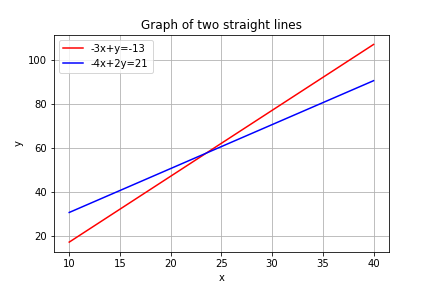
\includegraphics[width=\columnwidth]{./solutions/13/8/Figure1}
    \caption{Pair of straight lines for $k=-10$}
    \label{fig:solutions/13/8/figure1}
\end{figure}

Now Lets find equation of lines for $k=-\frac{35}{2}$.

Substitute $k=-\frac{35}{2}$ in \eqref{eq:solutions/13/8/1.1}. We get equation of pair of straight lines as:
\begin{align}
    12x^2-\frac{35}{2}xy+2y^2+11x-5y+2=0
\end{align}

%Comparing above equation with \eqref{eq:solutions/13/8/2.1}, we will get $a=12$, $b=-\frac{35}{4}$, $c=2$, $d=\frac{11}{2}$, $e=-\frac{5}{2}$, $f=2$.\\
From \eqref{eq:solutions/13/8/1.1}, \eqref{eq:solutions/13/8/2.3}, \eqref{eq:solutions/13/8/2.4} we get
\begin{align}
    \vec{V}=\vec{V}^T=\myvec{12 & -\frac{35}{4} \\ -\frac{35}{4} & 2}\label{eq:solutions/13/8/2.48}\\
    \vec{u}=\myvec{\frac{11}{2} \\ -\frac{5}{2}}\label{eq:solutions/13/8/2.49}
\end{align}
If $\mydet{\vec{V}}<0$ then two lines will intersect.
\begin{align}
    \mydet{\vec{V}}&=\mydet{12 & -\frac{35}{4} \\ -\frac{35}{4} & 2}\\
    \implies\mydet{\vec{V}}&=-\frac{841}{16}\\
    \implies\mydet{\vec{V}}&<0
\end{align}
Therefore the lines will intersect.\\
Now from \eqref{eq:solutions/13/8/conv},
\begin{align}
    \implies\vec{n_1}*\vec{n_2}&=\myvec{a \\ 2b \\c}=\myvec{12\\-\frac{35}{2}\\2}\label{eq:solutions/13/8/conv2}
\end{align}
The slopes of the lines are given by roots of equation \eqref{eq:solutions/13/8/poly}
\begin{align}
    \implies 2m^2-\frac{35}{2}m+12=0\\
    m_i=\frac{-b\pm{\sqrt{-\mydet{\vec{V}}}}}{c}\\
    \implies m_i=\frac{\frac{35}{4}\pm{\sqrt{\frac{841}{16}}}}{2}\\
    \implies m_1=8\\
     m_2=\frac{3}{4}
\end{align}
The normal vector for two lines is given by \eqref{eq:solutions/13/8/normvec}
\begin{align}
    \implies\vec{n_1}=k_1\myvec{-8\\1}\label{eq:solutions/13/8/n3}\\
    \vec{n_2}=k_2\myvec{-\frac{3}{4}\\1}\label{eq:solutions/13/8/n4}
\end{align}
Substituting \eqref{eq:solutions/13/8/n3},\eqref{eq:solutions/13/8/n4} in \eqref{eq:solutions/13/8/conv2}. we get
\begin{align}
    k_1k_2=2
\end{align}
The possible combinations of ($k_1$,$k_2$) are (1,2), (2,1), (-1,-2) and (-2,-1).\\
lets assume $k_1=1$,$k_2=2$ we get

\begin{align}
    \implies\vec{n_1}=\myvec{-8\\1}\label{soln3}\\
    \vec{n_2}=\myvec{-\frac{3}{2}\\2}\label{soln4}
\end{align}
We verify obtained $\vec{n_1}$,$\vec{n_2}$ using Toeplitz matrix
\begin{align}
    \vec{n_1}*\vec{n_2}=\myvec{-8 & 0\\1 & -8\\0 & 1}\myvec{-\frac{3}{2} \\ 2}=\myvec{12\\-\frac{35}{2}\\2}\\
    \implies\vec{n_1}*\vec{n_2}=\myvec{12\\-\frac{35}{2}\\2}=\myvec{a\\ 2b \\ c}
\end{align}
Therefore the obtained $\vec{n_1}$,$\vec{n_2}$ are correct.\\
Substitute \eqref{soln3}, \eqref{soln4} in \eqref{eq:solutions/13/8/1.16} we get 
\begin{align}
    c_2\myvec{-8\\1}+c_1\myvec{-\frac{3}{2}\\2}=\myvec{ -11\\ -5}
\end{align}
Solve using row reduction technique.
\begin{align}
    \implies\myvec{-\frac{3}{2} & -8 & -11\\2 & 1 & -5}\\
    \xleftrightarrow[]{R_1\leftarrow 2R_1}\myvec{-3 & -16 & -22\\2 & 1 & -5}\\
    \xleftrightarrow[]{R_2\leftarrow 3R_2+2R_1}\myvec{-3 & -16 & -22\\0 & -29 & -59}\\
    \xleftrightarrow[]{R_1\leftarrow 29R_1-16R_2}\myvec{-87 & 0 & 306\\0 & -29 & -59}\\
    \implies\myvec{1 & 0 & -\frac{102}{29}\\0 & 1 & \frac{59}{29}}\\
    \implies c_1=-\frac{102}{29}\label{c3}\\
    c_2=\frac{59}{29}\label{c4}
\end{align}

Substituting \eqref{soln3},\eqref{soln4},\eqref{c3},\eqref{c4} in \eqref{eq:solutions/13/8/1.12} and \eqref{eq:solutions/13/8/1.13}. we get equation of two straight lines.
\begin{align}
    \myvec{-8 & 1}\vec{x}=-\frac{102}{29}\\
    \myvec{-\frac{3}{2} & 2}\vec{x}=\frac{59}{29}
\end{align}
%\newpage
%The plot of these two lines is shown in Fig.~\ref{fig:solutions/13/8/figure2}.
%\begin{figure}[ht!]
%    \centering
%    \includegraphics[width=\columnwidth]{./solutions/13/8/Figure2}
%    \caption{Pair of straight lines for $k=-\frac{35}{2}$}
%    \label{fig:solutions/13/8/figure2}
%\end{figure}

%
\item Find the value of $k$ so that the following equation may represent a pair of straight lines - 
\begin{align}
6x^2 +xy+ky^2-11x+43y-35 = 0 \label{eq:solutions/13/94}
\end{align}
\solution
The given second degree equation is,
Comparing coefficients of \eqref{eq:solutions/13/94} we get,
\begin{align}
\vec{V} &= \myvec{6&\frac{1}{2}\\\frac{1}{2}&k}\\
\vec{u} &= \myvec{-\frac{11}{2}\\\frac{43}{2}}\\
f &= -35
\end{align}

The given second degree equation \eqref{eq:solutions/13/94} will represent a pair of straight line if, 
\begin{align}
\mydet{6&\frac{1}{2}&-\frac{11}{2}\\ \frac{1}{2}&k&\frac{43}{2}\\-\frac{11}{2}& \frac{43}{2}&-35}&=0\\
\intertext{Expanding the determinant,}
k+12&=0\\
\implies k&=-12\label{eq:solutions/13/95}
\end{align}
Hence, from \eqref{eq:solutions/13/95} we find that for $k=-12$, the given second degree equation \eqref{eq:solutions/13/94} represents pair of straight lines. For the appropriate value of $k$, \eqref{eq:solutions/13/94} becomes,
\begin{align}
6x^2 +xy-12y^2-11x+43y-35 = 0\label{eq:solutions/13/9main}
\end{align}

Let the pair of straight lines in vector form is given by
\begin{align}
    \vec{n_1}^T\vec{x}&=c_1\label{l1}\\
    \vec{n_2}^T\vec{x}&=c_2\label{l2}
\intertext{The pair of straight lines is given by,}
(\vec{n_1}^T\vec{x}-c_1)(\vec{n_2}^T\vec{x}-c_2) &=\vec{x}^T\vec{V}\vec{x}+2\vec{u^T}\vec{x}+f=0
\end{align}
Putting the values of $\vec{V}$ and $\vec{u}$ we get,
\begin{align}
\vec{x}^T\myvec{6&\frac{1}{2}\\\frac{1}{2}&-12}\vec{x}+2\myvec{-\frac{11}{2}&\frac{43}{2}}\vec{x}-35 &=0\label{eq:solutions/13/9line}
\end{align}
Hence, from \eqref{eq:solutions/13/9line} we get,
\begin{align}
\vec{n_1}*\vec{n_2}&=\myvec{6\\1\\-12}\label{eq:solutions/13/9conv}\\
c_2\vec{n_1}+c_1\vec{n_2}&=-2\myvec{-\frac{11}{2}\\\frac{43}{2}}\label{eq:solutions/13/9c1c2}\\
    c_1c_2&=-35
\end{align}
The slopes of the pair of straight lines are given by the roots of the polynomial,
\begin{align}
    &cm^2+2bm+a=0\label{eq:solutions/13/9quad}\\
    \implies m_i&=\frac{-b\pm{\sqrt{-\det(V)}}}{c}\\
    \vec{n_i}&=k\myvec{-m_i\\1}\label{eq:solutions/13/9slopes}
\end{align}
Substituting the values in above equations \eqref{eq:solutions/13/9quad} we get,
\begin{align}
    &-12m^2+m+6=0\\
    &\implies m_i=\frac{-\frac{1}{2}\pm{\sqrt{-(-\frac{289}{4})}}}{-12}\label{m}
\end{align}
Solving equation \eqref{m} we get ,
\begin{align}
    m_1&=-\frac{2}{3}\\
    m_2&=\frac{3}{4}\\
\intertext{Hence putting the values of $m_1$ and $m_2$ in \eqref{eq:solutions/13/9slopes} we get}
    \vec{n_1}&=k_1\myvec{\frac{2}{3}\\1}\label{eq:solutions/13/9n1}\\
    \vec{n_2}&=k_2\myvec{-\frac{3}{4} \\1}\label{eq:solutions/13/9n2}
\end{align}
Putting values of $\vec{n_1}$ and $\vec{n_2}$ in \eqref{eq:solutions/13/9conv} we get,
\begin{align}
\vec{n_1}*\vec{n_2} = \myvec{-\frac{3k_2}{4}&0\\k_2&-\frac{3k_2}{4}\\0&k_2}\myvec{\frac{2k_1}{3}\\k_1} &= \myvec{6\\1\\-12}\\
\implies\myvec{-\frac{1}{2}k_1k_2\\-\frac{1}{12}k_{1}k_{2}\\k_{1}k_{2}}&= \myvec{6\\1\\-12}\label{toeplizconv}
\end{align}
Thus, from \eqref{toeplizconv}, $k_{1}k_{2} = -12$. Possible combinations of ($k_1,k_2$) are (6,-2), (-6,2), (3,-4), (-3,4)
Lets assume $k_1=3$, $k_2=-4$, then we get, 
\begin{align}
    \vec{n_1}&=\myvec{2\\3}\label{eq:solutions/13/9n11}\\
    \vec{n_2}&=\myvec{3\\-4}\label{eq:solutions/13/9n22}
\end{align}
From equation \eqref{eq:solutions/13/9c1c2} we get 
\begin{align}
    \myvec{\vec{n_1} & \vec{n_2}}\myvec{c_2\\c_1}&=-2\vec{u}\\
    \myvec{2 & 3\\3 & -4}\myvec{c_2\\c_1}&=-2\myvec{-\frac{11}{2}\\\frac{43}{2}}\
\intertext{Hence we get the following equations,}
    2c_2+3c_1&=11\label{eq:solutions/13/9sol1}\\
    3c_2-4c_1&=-43\label{eq:solutions/13/9sol2}
\end{align}
The augmented matrix of \eqref{eq:solutions/13/9sol1} ,\eqref{eq:solutions/13/9sol2} is,
\begin{align}
\myvec{2&3&11\\3&-4&-43}&\underleftrightarrow{R_1=\frac{1}{2}R_1}\myvec{1&\frac{3}{2}&\frac{11}{2}\\3&-4&-43}\\
&\underleftrightarrow{R_2=R_2-3R_1}\myvec{1&\frac{3}{2}&\frac{11}{2}\\0&-\frac{17}{2}&-\frac{119}{2}}\\
&\underleftrightarrow{R_2=-\frac{2}{17}}\myvec{1&\frac{3}{2}&\frac{11}{2}\\0&1&7}\\
&\underleftrightarrow{R_1=R_1-\frac{3}{2}R_2}\myvec{1&0&-5\\0&1&7}\\
\end{align}
Hence we get,
\begin{align}
    c_1&=-5\\
    c_2&=7
\end{align}
Hence \eqref{l1}, \eqref{l2} can be modified as follows,
\begin{align}
    \myvec{2 & 3}\vec{x}&=-5\label{eq:solutions/13/9line1}\\
    \myvec{3 & -4}\vec{x}&=7\label{eq:solutions/13/9line2}
\end{align}
The figure below corresponds to the pair of straight lines represented by \eqref{eq:solutions/13/9line1} and \eqref{eq:solutions/13/9line2}.
\begin{figure}[h!]
\centering
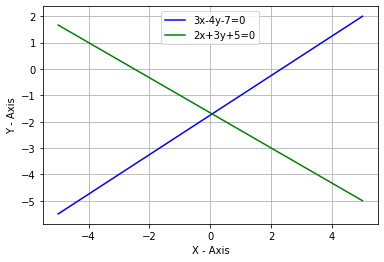
\includegraphics[width = \columnwidth]{./solutions/13/9/Lines.png}
\caption{Pair of Straight Lines}
\label{fig:solutions/13/9my_label}
\end{figure}


\item Find the value of k so that following equation may represent pairs of straight lines,
\begin{align}
kxy-8x+9y-12 = 0
\label{eq:solutions/13/10/Q_eq}
\end{align}
\solution
The general equation of second degree is given by,
\begin{align}
ax^2 + 2bxy + cy^2 + 2dx +2ey +f = 0
\label{eq:solutions/13/10/main_eq}
\end{align}
In vector from the equation \eqref{eq:solutions/13/10/main_eq} canb be expressed as,
\begin{align}
\vec{x}^T\vec{V}\vec{x} + 2\vec{u}^T\vec{x} + f = 0 
\label{eq:solutions/13/10/line_vec}
\end{align}
where,
\begin{align}
\vec{V} = \vec{V}^T = \myvec{a&b\\b&c}
\label{eq:solutions/13/10/vec1}
\end{align}
\begin{align}
\vec{u} = \myvec{d\\e}
\label{eq:solutions/13/10/vec2}
\end{align}
Now, comparing equation \eqref{eq:solutions/13/10/main_eq} to \eqref{eq:solutions/13/10/Q_eq} we get, a = c = 0, b = $\brak{\frac{k}{2}}$, d = -4, e = $\brak{\frac{9}{2}}$, f = -12.  
Hence, substituting these values in equation \eqref{eq:solutions/13/10/vec1} and \eqref{eq:solutions/13/10/vec2} we get,
\begin{align}
\vec{V} = \vec{V}^T = \myvec{0&\frac{k}{2}\\\frac{k}{2}&0}
\end{align}
\begin{align}
\vec{u} = \myvec{-4\\\frac{9}{2}}
\end{align}
Now equation \eqref{eq:solutions/13/10/Q_eq} represents pair of straight lines if,
\begin{align}
\mydet{\vec{V}&\vec{u}\\\vec{u}^T&f} = 0
\end{align}
\begin{align}
\mydet{0&\frac{k}{2}&-4\\\frac{k}{2}&0&\frac{9}{2}\\-4&\frac{9}{2}&-12} = 0
\end{align}
\begin{align}
\implies k =0 , k = 6 
\label{eq:solutions/13/10/k}
\end{align}
Substituting \eqref{eq:solutions/13/10/k} in \eqref{eq:solutions/13/10/Q_eq} we get,
\begin{align}
6xy-8x+9y-12 = 0
\end{align}
\begin{align}
-8x+9y-12 = 0
\end{align}
Hence value of k = 6 represents pair of straight lines.
Also it can be verified that the pair of lines intersect as,
\begin{align}
\mydet{\vec{V}} = \mydet{0&3\\3&0} <0 
\end{align} 
Let the pair of straight lines is given by,
\begin{align}
\vec{n_1}^T\vec{x} = c1
\label{eq:solutions/13/10/e1}
\end{align}
\begin{align}
\vec{n_2}^T\vec{x} = c2
\label{eq:solutions/13/10/e2}
\end{align}
Now equating the product of equation \eqref{eq:solutions/13/10/e1} and \eqref{eq:solutions/13/10/e2} with \eqref{eq:solutions/13/10/line_vec} we get,
\begin{align}
(\vec{n_1}^T\vec{x} - c1)(\vec{n_2}^T\vec{x} - c2) = \\\vec{x}^T\myvec{0&3\\3&0}\vec{x} + 2\myvec{-4& \frac{9}{2}}\vec{x} - 12 
\end{align}
\begin{align}
\implies n_1 * n_2 = \{0,6,0\}
\label{eq:solutions/13/10/verify}
\end{align}
\begin{align}
c_1n_1+c_2n_2 = \myvec{8\\-9}
\label{eq:solutions/13/10/sub1}
\end{align}
\begin{align}
c_1c_2 = -12.
\end{align}
Now the slopes of line is given by roots of polynomial,
\begin{align}
cm^2 + 2bm + a = 0
\end{align} 
\begin{align}
\implies 2bm = 0
\end{align}
\begin{align}
\implies m = 0
\end{align}
Also
\begin{align}
m_i = \frac{-b\pm\sqrt{-|V|}}{c} 
\end{align}
\begin{align}
\implies m_i = \frac{-0\pm\sqrt{9}}{0} 
\end{align}
\begin{align}
\therefore m_1 = 0
\end{align}
\begin{align}
 m_2 = \infty
\end{align}
The normal vector to the two lines is given by,
\begin{align}
n_i = k_i\myvec{-m_i\\1}
\end{align}
\begin{align}
\implies n_1 = k_1\myvec{0\\1}
\end{align}\\
\begin{align}
n_2 = k_2\myvec{1\\0}
\end{align}
Also,
\begin{align}
k_1k_2 = 6
\end{align}
Let $k_1$ = 2 and $k_2$ =3
\begin{align}
\implies n_1 = \myvec{0\\2}
\label{eq:solutions/13/10/n1}
\end{align}
\begin{align}
n_2 = \myvec{3\\0}
\label{eq:solutions/13/10/n2}
\end{align}
We verify obtained $n_1$ and $n_2$ using Toeplitz matrix,
\begin{align}
n_1*n_2 = \myvec{0&0\\2 &0\\0&2}\myvec{2\\0}\myvec{3\\0} = \myvec{0\\6\\0}
\label{eq:solutions/13/10/verify1}
\end{align}
Hence \eqref{eq:solutions/13/10/verify} and \eqref{eq:solutions/13/10/verify1} are same. Hence verified. 

Now substituting it in \eqref{eq:solutions/13/10/sub1} we get,
\begin{align}
c_2\myvec{0\\2}+c_1\myvec{3\\0} = \myvec{8\\-9}
\end{align}

Solve using Row reduction Technique we get,
\begin{align}
\implies\myvec{3&0&8\\0&2&-9} 
\end{align}

\begin{align}
\xleftrightarrow[]{R_1\leftarrow R_1/3}\myvec{1&0&8/3\\0&2&-9}
\end{align}
\begin{align}
\xleftrightarrow[]{R_2\leftarrow R_2/2}\myvec{1&0&8/3\\0&1&-9/2}
\end{align}
\begin{align}
\implies c_1 = \frac{8}{3}
\end{align}
\begin{align}
c_2 = \frac{-9}{2}
\end{align}
\begin{figure}[ht!]
\centering
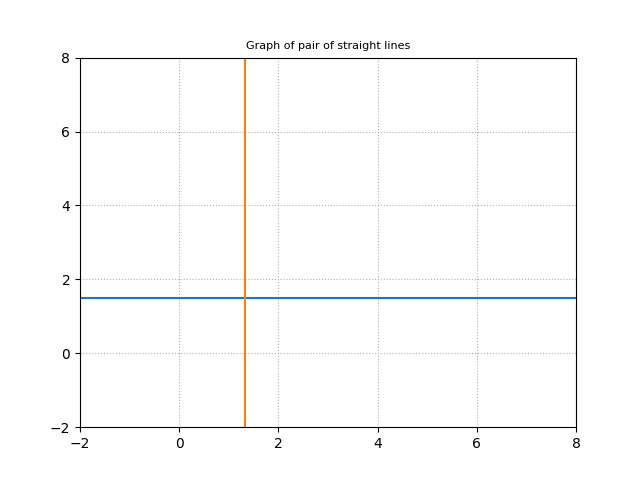
\includegraphics[width=\columnwidth]{./solutions/13/10/Figure_1.png}
\caption{Intersection of 2 lines}
\label{eq:solutions/13/10/Figure_1}
\end{figure}
substituting the values of $c_1$, $c_2$ and equation \eqref{eq:solutions/13/10/n1} and \eqref{eq:solutions/13/10/n2} to equation \eqref{eq:solutions/13/10/e1} and \eqref{eq:solutions/13/10/e2} we get equation of two straight lines.
\begin{align}
\implies \myvec{0&2}\vec{x} = \frac{8}{3}
\end{align}
\begin{align}
\myvec{3&0}\vec{x} = \frac{-9}{2}
\end{align}
Hence the equation of pair of straight lines are,
\begin{align}
\brak{\myvec{0&2}\vec{x}-\frac{8}{3}}\brak{\myvec{3&0}\vec{x} - \frac{-9}{2}} = 0
\label{eq:solutions/13/10/pair}
\end{align}
Hence, Plot of the equation \eqref{eq:solutions/13/10/pair} is shown in Figure.\ref{eq:solutions/13/10/Figure_1}
Now for value of k = 0 does not represent pair of straight lines.as,
\begin{align}
\mydet{\vec{V}} = \mydet{0&0\\0&0} \nless0 
\end{align} 
Hence, Plot of the equation $\myvec{-8&9}\vec{x} = 12$ is shown in figure \ref{eq:solutions/13/10/Figure_2},
\begin{figure}[ht!]
\centering
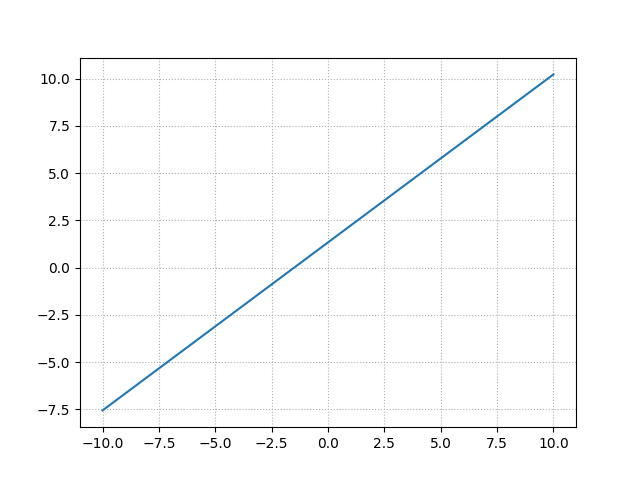
\includegraphics[width=\columnwidth]{./solutions/13/10/Figure_2.png}
\caption{Intersection of 2 lines}
\label{eq:solutions/13/10/Figure_2}
\end{figure}


\item Find the value of k such that 
\begin{align}
x^{2}+ \frac{10}{3}(xy)+y^2 -5x -7y + k =0 \label{eq:solutions/13/11eq5}
\end{align}
 represent pairs of straight lines.
\\
\solution
From  \eqref{eq:solutions/13/11eq5},
\begin{align}
	\vec{V} = \myvec{1& \frac{5}{3} \\ \frac{5}{3} & 1}\label{myeq:solutions/13/11/}\\
	\vec{u}^T = \myvec{\frac{-5}{2} & \frac{-7}{2}}\label{df:solutions/13/11/}
\end{align}
and
\begin{align}\label{eq:solutions/13/11/dett}
\mydet{1& \frac{5}{3} & \frac{-5}{2} \\ \frac{5}{3} & 1 & \frac{-7}{2} \\ \frac{-5}{2} & \frac{-7}{2} & k} = 0 \\
\implies \brak{k - \brak{\frac{49}{4}}}-\frac{5}{3}\brak{\frac{5}{3}k - \frac{35}{4}} \nonumber\\
-
\frac{5}{2} \brak{\frac{-35}{6}+\frac{5}{2}} = 0\\
\implies \frac{64}k{36} - \frac{128}{12} = 0\\
\implies \boxed{k = 6} \label{eq:solutions/13/11result}
\end{align}
Substituting \eqref{eq:solutions/13/11result} in \eqref{eq:solutions/13/11eq5}, we get
\begin{align}
	x^{2}+ \frac{10}{3}(xy)+y^2 -5x -7y + 6 =0  \label{eq:solutions/13/11reseq}
\end{align}
Hence value of k=6 represents pair of straight lines.
Substituting value of k =6 in \eqref{eq:solutions/13/11/dett}
\begin{align}
\delta&=\begin{array}{|ccc|}
1 &\frac{5}{3}& \frac{-5}{2}\\\frac{5}{3} & 1 & \frac{-7}{2}\\ \frac{-5}{2} & \frac{-7}{2} & 6
\end{array}&
\intertext{Simplyfying  the above determinant , we get}
\delta&=0
\end{align}
%Since equation \eqref{eq:solutions/13/11det1} is satisfied, we could say that the given equation 
\eqref{eq:solutions/13/11reseq} represents two straight lines
\begin{align}
    \det(V)&=\begin{array}{|cc|}
1&\frac{5}{3}\\\frac{5}{3} & 1
\end{array}<0
\end{align}
Since $\det(V)<0$  lines would intersect each other
\begin{figure}[h]
    \centering
    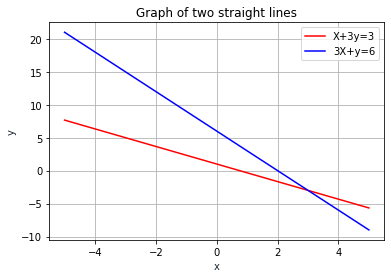
\includegraphics[width=\columnwidth]{./solutions/13/11/assignment5.png}
    \caption{Pair of straight lines}
    \label{Fig:solutions/13/11/1}
\end{figure}
%pair of straight lines in vector form is :
%\begin{align}
%    \vec{n_1}^T\vec{x}&=c_1\label{eq:solutions/13/11/m1}\\
%    \vec{n_2}^T\vec{x}&=c_2\label{eq:solutions/13/11/m2}
%\end{align}
%Equating their product with \eqref{eq:solutions/13/11eq4}
%\begin{align}
%(\vec{n_1}^T\vec{x}-c_1)(\vec{n_2}^T\vec{x}-c_2) &=\vec{x}^T\myvec{1 & \frac{5}{3} \\\frac{5}{3} & 1}\vec{x}\notag\\
%+2\myvec{\frac{-5}{2} & \frac{-7}{2}}\vec{x}+6\label{eq:solutions/13/11/86}
%\end{align}
\begin{align}
    \vec{n_1}*\vec{n_2}&=\{1,\frac{10}{3},1\}\label{eq:solutions/13/11/conv}\\
    c_2\vec{n_1}+c_1\vec{n_2}&=-2\myvec{\frac{-5}{2}\\\frac{-7}{2}}\label{eq:solutions/13/11/eq98}\\
    c_1c_2&=6
\end{align}
The slopes of the lines are given by the roots of the polynomial 
\begin{align}
    &cm^2+2bm+a=0\label{eq:solutions/13/11/e}\\
    \implies m_i&=\frac{-b\pm{\sqrt{-\det(V)}}}{c}\\
    \vec{n_i}&=k\myvec{-m_i\\1}
\end{align}
Substituting  in above equations \eqref{eq:solutions/13/11/e} we get,
\begin{align}
    &m^2+\frac{10}{3}m+1=0\\
    &\implies m_i=\frac{\frac{-10}{3}\pm{\sqrt{-(\frac{-16}{9})}}}{1}\label{eq:solutions/13/11/eq12}
\end{align}
Solving equation \eqref{eq:solutions/13/11/eq12} we have ,
\begin{align}
    m_1&=\frac{-1}{3}\\
    m_2&=-3\\
    \vec{n_1}&=k_1\myvec{\frac{1}{3}\\1}\label{eq:solutions/13/11/n1}\\
    \vec{n_2}&=k_2\myvec{{3}\\1}\label{eq:solutions/13/11/n2}
\end{align}
Substituting equations \eqref{eq:solutions/13/11/n1}, \eqref{eq:solutions/13/11/n2} in equation \eqref{eq:solutions/13/11/conv} we get 
\begin{align}
    k_1k_2&=1
\end{align}
Possible combination of ($k_1,k_2$) is (1,1)
Lets assume $k_1=1$, $k_2=1$, we get 
\begin{align}
    \vec{n_1}&=\myvec{\frac{1}{3} \\1}\label{eq:solutions/13/11/n11}\\
    \vec{n_2}&=\myvec{3\\1}\label{eq:solutions/13/11/n22}
\end{align}
we have:
\begin{align}
\vec{n_1}\ast \vec{n_2} = \myvec{a\\2b\\c} \label{eq:solutions/13/11conv1}
\end{align}
Convolution of $\vec{n_1}$ and $\vec{n_2}$ can be done by converting  $\vec{n_1}$ into a teoplitz matrix and multiplying with $\vec{n_2}$\\
From equation \eqref{eq:solutions/13/11/n11} and \eqref{eq:solutions/13/11/n22}
\begin{align}
    \vec{n_1}=\myvec{\frac{1}{3}&0\\1&\frac{1}{3}\\0&1}
    \vec{n_2}=\myvec{3\\ 1}\label{eq:solutions/13/11conv2}\\
\implies \myvec{\frac{1}{3}&0\\1&\frac{1}{3}\\0&1}\myvec{3\\ 1} = \myvec{1\\\frac{10}{3}\\1} = \myvec{a\\2b\\c}\label{eq:solutions/13/11conv3}
\end{align}
$c_1$ and $c_2$ can be obtained as,
\begin{align}
\myvec{\vec{n_1} & \vec{n_2}}\myvec{c_2\\c_1}&=-2\vec{u}\\
\myvec{\vec{n_1} & \vec{n_2}}\myvec{c_2\\c_1}&=-2\myvec{\frac{-5}{2}\\\frac{-7}{2}}
\label{eq:solutions/13/11aug1}
\end{align}
Substituting \eqref{eq:solutions/13/11/n11} and \eqref{eq:solutions/13/11/n22} in \eqref{eq:solutions/13/11aug1}, the augmented matrix is,
\begin{align}
\myvec{\frac{1}{3} & 3& 5 \\ 1 & 1 & 7}
\xleftrightarrow[]{R_1 \leftarrow 3\times R_1}
\myvec{1 & 9&15\\ 1 & 1 & 7}
\end{align}
\begin{align}
\myvec{1 & 9&15\\ 1 & 1 & 7}
\xleftrightarrow[]{R_2 \leftarrow R_2- R_1}
\myvec{1 & 9&15\\ 0 & -8 & -8}
\end{align}
\begin{align}
\myvec{1 & 9&15\\ 0 & -8 & -8}
\xleftrightarrow[]{R_2 \leftarrow R_2\div -8}
\myvec{1 & 9&15\\ 0 & 1 & 1}
\end{align}
\begin{align}
\myvec{1 & 9&15\\ 0 & 1 & 1}
\xleftrightarrow[]{R_1 \leftarrow R_1-9\times R_2}
\myvec{1 & 0&6\\ 0 & 1&1 }
\end{align}
From above  we get 
\begin{align}
    c_1&=1\\
    c_2&=6
\end{align}
Hence pair of straight lines  are
%from  \eqref{eq:solutions/13/11/m1}, \eqref{eq:solutions/13/11/m2} in vector form
\begin{align}
    \myvec{\frac{1}{3}& 1}\vec{x}&=1\\
    \myvec{3 & 1}\vec{x}&=6
\end{align}

   

\item Prove that the equation
\begin{align}
	12x^2 + 7xy -10y^2 +13x +45y -35 =0 
\end{align}
represents two straight lines and find the angle between the lines.
\\
\solution
The above equation can be expressed as
\begin{align}
        \vec{x}^{T}\vec{Vx} + 2\vec{u}^{T}\vec{x} + f=0   \label{eq:solutions/13/12/eq2}
\end{align}
where
\begin{align}
	\vec{V}=\vec{V}^T &= \myvec{12 & \frac{7}{2} \\ \frac{7}{2} & -10} \\
	\vec{u} &= \myvec{\frac{13}{2} \\ \frac{45}{2}} \\
	 f=-35
\end{align}	
	(\ref{eq:solutions/13/12/eq2}) represents a pair of straight lines if
\begin{align}
	&\mydet{\vec{V} & \vec{u} \\ \vec{u}^T & f} = 0     \label{eq:solutions/13/12/eq5} \\
	\mydet{\vec{V} & \vec{u} \\ \vec{u}^T & f} 
		&= \mydet{12 & \frac{7}{2}  & \frac{13}{2} \\ 
	        \frac{7}{2} & -10 & \frac{45}{2}     \\
	       \frac{13}{2} & \frac{45}{2} & -35 }  \\
	       		\nonumber \\
	\implies \ 12\mydet{-10 & \frac{45}{2} \\ \frac{45}{2} & -35} 
		& -\frac{7}{2}\mydet{\frac{7}{2} & \frac{45}{2} \\ \frac{13}{2} & -35} 
		+\frac{13}{2}\mydet{\frac{7}{2} & -10 \\ \frac{13}{2} & \frac{45}{2}} = 0 \label{eq:solutions/13/12/eq10}\\
\end{align}
The lines intercept if
\begin{align}
        \mydet{\vec{V}} < 0 \\
 	\mydet{\vec{V}}=-\frac{529}{4} < 0 \label{eq:solutions/13/12/eq11}
\end{align}
From (\ref{eq:solutions/13/12/eq10}) and (\ref{eq:solutions/13/12/eq11}) it can be concluded that the given equation represents a pair of intersecting lines.
Let the equations of lines be
\begin{align}
	\vec{n_1}^T \vec{x}=c_1 \\
	\vec{n_2}^T \vec{x}=c_2 
\end{align}
Since (\ref{eq:solutions/13/12/eq2}) represents a pair of straight lines it must satisfy
\begin{align}
	(\vec{n_1}^T \vec{x} - c_1)(\vec{n_1}^T \vec{x} - c_1) =
        \vec{x}^{T}\vec{Vx} + 2\vec{u}^{T}\vec{x} + f=0
\end{align}
where
\begin{align}
	\vec{n_1}*\vec{n_2}=\myvec{a\\2b\\c}=\myvec{12\\7\\-10} \label{eq:solutions/13/12/eq6} \\ 
	c_2\vec{n_1}+c_1\vec{n_2}=-2\vec{u} \label{eq:solutions/13/12/eq9}\\
	c_1c_2=f
\end{align}
Slopes of the lines can be obtained by solving 
\begin{align}
	cm^2+2bm+a=0 \\
	-10m^2+7m+12=0 \\
	\implies m_1 = \frac{-4}{5}, m_2 = \frac{3}{2}
\end{align}
The normal vectors can be expressed in terms of corresponding slopes of lines as
\begin{align}
	\vec{n}=k\myvec{-m\\1} \\
	\implies
	\vec{n_1}=k_1\myvec{\frac{4}{5} \\ 1}  \label{eq:solutions/13/12/eq7} \\
	\vec{n_2}=k_2\myvec{-\frac{3}{2} \\ 1}  \label{eq:solutions/13/12/eq8}
\end{align}
Substituing (\ref{eq:solutions/13/12/eq7}) and (\ref{eq:solutions/13/12/eq8}) in (\ref{eq:solutions/13/12/eq6}) we get
\begin{align}
	k_1k_2=-10
\end{align}
Assuming $ k_1=5$ and $k_2 =-2$
\begin{align}
	\vec{n_1}=\myvec{4\\5}, \vec{n_2}=\myvec{3\\-2}
\end{align}
Verification using Toeplitz matrix
\begin{align}
\vec{n_1}*\vec{n_2}=\myvec{4 & 0 \\ 5 & 4 \\0 & 5}\myvec{3\\-2}=\myvec{12\\7\\-10}
\end{align}
From (\ref{eq:solutions/13/12/eq9}) we have
\begin{align}
	c_2\myvec{4\\5}+c_1\myvec{3\\-2}=\myvec{-13\\-45}
\end{align}
Solving the augmented matrix
\begin{align}
	\myvec{4 & 3 & -13 \\ 5 & -2 & -45}
	\xleftrightarrow[]{R_2 \leftarrow 4R_2-5R_1}
	\myvec{4 & 3 & -13 \\ 0 & -23 & -115}\\
	\xleftrightarrow[]{R_2 \leftarrow -\frac{R_2}{23}}
        \myvec{4 & 3 & -13 \\ 0 & 1 & 5}
        \xleftrightarrow[]{R_1 \leftarrow R_1-3R_2}
	\myvec{4 & 0 & -28 \\ 0 & 1 & 5}\\
	\xleftrightarrow[]{R_1 \leftarrow \frac{R_1}{4}}
        \myvec{1 & 0 & -7 \\ 0 & 1 & 5} \\
	\implies \quad c_1 =-7, \ c_2 =5
\end{align}
Thus the equation of lines are
\begin{align}
	\myvec{4 & 5}\vec{x} = 5 \\
	\myvec{3 & -2}\vec{x} = -7 
\end{align}
The angle between the lines can be expressed interms of normal vectors 
\begin{align}
	\vec{n_1}=\myvec{4\\5} , \quad \vec{n_2}=\myvec{3\\-2}
\end{align}
as
\begin{align}
	\cos\theta=\frac{\vec{n_1}^T\vec{n_2}}{\norm{\vec{n_1}}\norm{\vec{n_2}}} \\
				\nonumber \\
	\implies \quad \theta=\cos^{-1}({\frac{2}{\sqrt{533}}}) = \tan^{-1}(\frac{23}{2})
\end{align}
\begin{figure}[!h]
	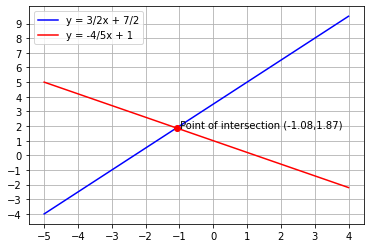
\includegraphics[width=\columnwidth]{./solutions/13/12/lines.png}
	\caption{} \label{eq:solutions/13/12/linefig1}
\end{figure}


\item Find the value of k so that the following equation may represent the pair of staright lines:
\begin{align}
	2x^2+ xy -y^2 + kx + 6y - 9 = 0 \label{eq:solutions/13/13/1} 
\end{align}

\solution
We need to find the value of k for which \eqref{eq:solutions/13/13/1} represents a pair of straight lines.

Converting \eqref{eq:solutions/13/13/1} into vector form, we get
\begin{align}
	\vec{x}^T\myvec{2 & 1/2 \\ 1/2 & -1}\vec{x}+2\myvec{k/2 \\ 3}\vec{x}-9=0 \label{eq:solutions/13/13/2}
\end{align} 
Here, we have
\begin{align}
& \vec{V} = \vec{V}^T = \myvec{2 & 1/2 \\ 1/2 & -1} \\
& \vec{u} = \myvec{k/2 \\ 3} \\
& f = -9
\end{align}
The above represents a pair of straight lines if
\begin{align}
	\begin{array}{|cc|}
		\vec{V} & \vec{u}\\\vec{u}^T & f
	\end{array}&=0\label{eq:solutions/13/13/3}
\end{align}
Since \eqref{eq:solutions/13/13/1} represents a pair of straight lines, then by \eqref{eq:solutions/13/13/3}, we have
\begin{align}
	\begin{array}{|ccc|}
		2 & 1/2 & k/2 \\ 1/2 & -1 & 3  \\ k/2 & 3 & -9 
	\end{array}&=0
\end{align}
By solving, above determinant we get
\begin{align}
& 2(9-9) + \frac{-1}{2}(\frac{-9}{2} + \frac{-3k}{2}) + \frac{k}{2}(\frac{3}{2} + \frac{k}{2})  = 0\\
& \frac{(9+3k)}{4} + \frac{k(3+k)}{4}  = 0 \\
& k^2 + 6k + 9 =0 \\
& (k+3)^2 = 0 \\
& k = -3 \label{eq:solutions/13/13/4}
\end{align}
Hence by \eqref{eq:solutions/13/13/4}, we have
\begin{align}
   2x^2+ xy -y^2 - 3x + 6y - 9 &= 0
\end{align} 
represents family of straight lines for $k=-3$.


To find the staright lines, we write each of thrm in their vector form as
\begin{align}
	& \vec{n_1}^T\vec{x} =c_1 \\
	& \vec{n_2}^T\vec{x} =c_2 
\end{align} 
Equating the product of above with \eqref{eq:solutions/13/13/2}, we have
\begin{multline}
 \brak{\vec{n_1}^T\vec{x}-c_1}\brak{\vec{n_2}^T\vec{x}-c_2} = \\ 
\vec{x}^T\myvec{2 & 1/2 \\ 1/2 & -1}\vec{x}+2\myvec{k/2 \\ 3}\vec{x}-9
\end{multline}
\begin{align}
\implies & \vec{n_1}*\vec{n_2} = \myvec{2 \\ 1 \\ -1}\label{eq:solutions/13/13/5} \\
& c_2\vec{n_1} + c_1\vec{n_1} =-2\myvec{-3/2 \\ 3}\label{eq:solutions/13/13/6} \\
& c_1c_2 = -9 \label{eq:solutions/13/13/7}
\end{align}
Here, the slope of these lines are given by the roots of the polynomial
\begin{align}
-& m^2 + m + 2 = 0 \\ 
 & m^2 - m - 2 = 0 \\
 & m = \frac{1 \pm \sqrt{1+8}}{2} \\
 & m_1 = \frac{1+3}{2} = 2 \\
 & m_2 = \frac{1-3}{2} = -1 \\
 & n_1 = k_1\myvec{-2 \\ 1}\label{eq:solutions/13/13/8} \\
 & n_2 = k_2\myvec{1 \\ 1}\label{eq:solutions/13/13/9}
\end{align}
Substituing \eqref{eq:solutions/13/13/8} and \eqref{eq:solutions/13/13/9} in \eqref{eq:solutions/13/13/5}, we get
\begin{align}
	k_1k_2 = -1
\end{align}
Taking $k_1=-1$ and $k_2=1$, we get
\begin{align}
	& n_1 = \myvec{2 \\ -1} \\
	& n_2 = \myvec{1 \\ 1}
\end{align}
Substituting in \eqref{eq:solutions/13/13/6} for  above values of$n_1$ and $n_2$
\begin{align}
& \myvec{ n_1 n_2} \myvec{c_2 \\ c_1} \quad= \myvec{3\\-6} \\
& \myvec{2 &1 \\ -1 &1} \myvec{c_2 \\ c_1} = \myvec{3\\-6}\label{eq:solutions/13/13/10}
\end{align}
Solving \eqref{eq:solutions/13/13/10},
\begin{multline}
\myvec{2 &1 \\ -1 &1} \myvec{c_2 \\ c_1} = \myvec{3\\-6} \xLeftrightarrow[]{r_2 = r_2 + 2r_1} \\
\myvec{2 &1 \\ 0 &3} \myvec{c_2 \\ c_1} = \myvec{3\\-9}
\end{multline}
\begin{multline}
	\myvec{2 &1 \\ 0 &3} \myvec{c_2 \\ c_1} = \myvec{3\\-9} \xLeftrightarrow[]{r_2 = r_2/3} \\
	\myvec{2 &1 \\ 0 &1} \myvec{c_2 \\ c_1} = \myvec{3\\-3}
\end{multline}
\begin{multline}
	\myvec{2 &1 \\ 0 &1} \myvec{c_2 \\ c_1} = \myvec{3\\-3} \xLeftrightarrow[]{r_1 = r_1-r_2} \\
	\myvec{2 &0 \\ 0 &1} \myvec{c_2 \\ c_1} = \myvec{6\\-3}
\end{multline}
Hence, we found out
\begin{align}
	&c_1 = -3 \\
	&c_2 = 3
\end{align}
Thus, pair of staright lines are
\begin{align}
& \myvec{2 &-1}\vec{x} = -3 \\
& \myvec{1 &1}\vec{x} = 3 
\end{align}
where
\begin{align}
\vec{x} = \myvec{x \\ y}	
\end{align}
The plot of above is shown below 
\begin{figure}[!htb]
	
	\centering
	
	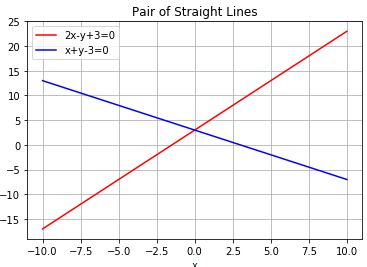
\includegraphics[width=\columnwidth]{./solutions/13/13/Latex/assignment4fig.jpg}
	
	\caption{Pair of Straight Lines}
	
	\label{eq:solutions/13/13/fig:1}
	
\end{figure}


%
\item Prove that the equation $12x^2+7xy-10y^2+13x+45y-35=0$ represents two straight lines and find the angle between them. 
\\
\solution
The general second order equation is given by ,
\begin{align}
ax^2+2bxy+cy^2+2dx+2ey+f&=0\label{eq:solutions/13/ex1/eq1}
\end{align}
Given,
\begin{align}
    12x^2+7xy-10y^2+13x+45y-35&=0 \label{eq:solutions/13/ex1/eqgiven}
\end{align}
The above equation can be expressed as
\begin{align}
        \vec{x}^{T}\vec{Vx} + 2\vec{u}^{T}\vec{x} + f=0   \label{eq:solutions/13/ex1/eq:solutions/eq2}
\end{align}
where
\begin{align}
	\vec{V}=\vec{V}^T &= \myvec{12 & \frac{7}{2} \\ \frac{7}{2} & -10} \\
	\vec{u} &= \myvec{\frac{13}{2} \\ \frac{45}{2}} \\
	 f=-35
\end{align}	
	(\ref{eq:solutions/13/ex1/eq:solutions/eq2}) represents a pair of straight lines if
\begin{align}
	&\mydet{\vec{V} & \vec{u} \\ \vec{u}^T & f} = 0     \label{eq:solutions/13/ex1/eq:solutions/eq5} \\
	\mydet{\vec{V} & \vec{u} \\ \vec{u}^T & f} 
		&= \mydet{12 & \frac{7}{2}  & \frac{13}{2} \\ 
	        \frac{7}{2} & -10 & \frac{45}{2}     \\
	       \frac{13}{2} & \frac{45}{2} & -35 }  \\
	       		\nonumber \\
	\implies \ 12\mydet{-10 & \frac{45}{2} \\ \frac{45}{2} & -35} 
		& -\frac{7}{2}\mydet{\frac{7}{2} & \frac{45}{2} \\ \frac{13}{2} & -35} 
		+\frac{13}{2}\mydet{\frac{7}{2} & -10 \\ \frac{13}{2} & \frac{45}{2}} = 0 \label{eq:solutions/13/ex1/eq:solutions/eq10}
\end{align}
The lines intercept if
\begin{align}
        \mydet{\vec{V}} < 0 \\
 	\mydet{\vec{V}}=-\frac{529}{4} < 0 \label{eq:solutions/13/ex1/eq:solutions/eq11}
\end{align}
\renewcommand{\thefigure}{1}
From (\ref{eq:solutions/13/ex1/eq:solutions/eq10}) and (\ref{eq:solutions/13/ex1/eq:solutions/eq11}) it can be concluded that the given equation represents a pair of intersecting lines.\\
Let $(\alpha,\beta)$ be their point of intersection, then
\begin{align}
	\label{eq:solutions/13/ex1/eq16}\myvec{ 12 & \frac{7}{2}\\\frac{7}{2} & -10}\myvec{\alpha \\ \beta} = \myvec{\frac{-13}{2} \\ -\frac{45}{2}} \\
	\label{eq:solutions/13/ex1/eq17}\implies \myvec{\alpha \\ \beta} = \myvec{-1 \\ 2}
\end{align}
\begin{equation}
	\text{From \textit{Spectral theorem, }}\vec{V} = \vec{P}\vec{D}\vec{P}^T
\end{equation}
\begin{align}
	\label{eq:solutions/13/ex1/eq18}\vec{V} &= \myvec{ 12 & \frac{7}{2}\\ \frac{7}{2} & -10}\\
	\label{eq:solutions/13/ex1/eq19}\vec{P} &= \myvec{\frac{-\sqrt{533} - 22}{2} & \frac{-22 + \sqrt{533}}{2}\\ 1 & 1}\\
	\label{eq:solutions/13/ex1/eq20}\vec{D} &= \myvec{1 + \frac{\sqrt{533}}{2} & 0\\ 0 & 1 - \frac{\sqrt{533}}{2}}
\end{align}
Using \textit{Spectral decomposition} of matrix we can express equation as
\begin{align}
	\label{eq:solutions/13/ex1/eq14}u_1(x-\alpha) + u_2(y-\beta) &= \pm \sqrt{-\frac{\lambda_2}{\lambda_1}}(v_1(x-\alpha) + v_2(y-\beta))
\end{align}
Substituting values in above equation we get;
\begin{multline}\label{eq:solutions/13/ex1/eq21}
	\frac{\sqrt{533}-22}{2}(x+1) + (y-2) \\= \pm \sqrt{-\frac{1 - \frac{\sqrt{533}}{2}}{1 + \frac{\sqrt{533}}{2}}}\left(\frac{-22 -\sqrt{533}}{2}(x+1) + (y-2)\right)
\end{multline}
Simplifying \eqref{eq:solutions/13/ex1/eq21},
\begin{align}
	\label{eq:solutions/13/ex1/eq22}3x -2y + 7 = 0 \text{ and } 4x + 5y -5 = 0\\
	\implies (3x - 2y + 7)(4x + 5y - 5) = 0
\end{align}
Thus the equation of lines are
\begin{align}
	\myvec{4 & 5}\vec{x} = 5 \\
	\myvec{3 & -2}\vec{x} = -7 
\end{align}
\begin{figure}[h]
    \centering
    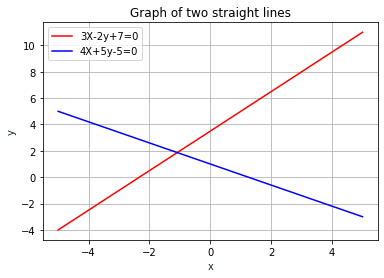
\includegraphics[width=\columnwidth]{./solutions/13/ex1/Figure.png}
    \caption{Pair of straight lines}
    \label{eq:solutions/13/ex1/Fig :1}
\end{figure}
{Angle between the straight lines: }
The angle between the lines can be expressed in terms of normal vectors 
\begin{align}
	\vec{n_1}=\myvec{4\\5} , \quad \vec{n_2}=\myvec{3\\-2}
\end{align}
\begin{align}
	\cos\theta=\frac{\vec{n_1}^T\vec{n_2}}{\norm{\vec{n_1}}\norm{\vec{n_2}}} \\
				\nonumber \\
	\implies \quad \theta=\cos^{-1}({\frac{2}{\sqrt{533}}}) = \tan^{-1}(\frac{23}{2})
\end{align}

\item Find the value of $h$ so that the equation 
\begin{align}
6x^2+2hxy+12y^2+22x+31y+20=0
\label{eq:solutions/13/ex2/question}
\end{align}
 may represent two straight lines.
\\
\solution
The general equation second degree is given by
\begin{equation}\label{eq:solutions/13/ex2/eq1}
	ax^2 + 2bxy + cy^2 + 2dx + 2ey + f = 0
\end{equation}
\eqref{eq:solutions/13/ex2/eq1} represents pair of straight lines if
\begin{equation}\label{eq:solutions/13/ex2/eq2}
	\mydet{ a & h & d\\
			h & c & e\\
			d & e & f} = 0
\end{equation}
From \eqref{eq:solutions/13/ex2/eq2}, given equation represents pair of straight lines if 
\begin{equation}\label{eq:solutions/13/ex2/eq3}
	\mydet{ 6 & h & 11\\
			h & 12 & \frac{31}{2}\\
			11 & \frac{31}{2} & 20} = 0
\end{equation}
\begin{equation}\label{eq:solutions/13/ex2/eq4}
	\implies h = \frac{17}{2} \text{ or } h = \frac{171}{20}
\end{equation}
Verify  \eqref{eq:solutions/13/ex2/eq4} using python code from
\begin{lstlisting}
https://github.com/shreeprasadbhat/matrix-theory/tree/master/assignment5/codes/solve_determinant.py
\end{lstlisting}
The general equation second degree is given by
\begin{equation}\label{eq:solutions/13/ex2/eq5}
	ax^2 + 2bxy + cy^2 + 2dx + 2ey + f = 0
\end{equation}
Let $(\alpha,\beta)$ be their point of intersection, then
\begin{equation}\label{eq:solutions/13/ex2/eq6}
	\myvec{ a & h\\ h & b}\myvec{\alpha \\ \beta} = \myvec{-d \\ -e}
\end{equation}
Under \textit{Affine transformation},
\begin{align}
	\vec{x} &= \vec{M}\vec{y} + c\\
	\myvec{x \\ y} &= \myvec{1 & 0 \\ 0 & 1} \myvec{X \\ Y} + \myvec{\alpha \\ \beta}\\
	\label{eq:solutions/13/ex2/eq7}\myvec{x \\ y} &= \myvec{X+\alpha \\ Y+\beta}
\end{align}
\eqref{eq:solutions/13/ex2/eq5} under transformation \eqref{eq:solutions/13/ex2/eq7} will become,
\begin{equation}\label{eq:solutions/13/ex2/eq8}
	aX^2 + 2bXY + cY^2 = 0
\end{equation}
\begin{equation}\label{eq:solutions/13/ex2/eq9}
	\myvec{X & Y} \myvec{a & h \\ h & b} \myvec{X \\ Y} = 0
\end{equation}
%\begin{equation}\label{eq:solutions/13/ex2/eq10}
%	\vec{X}^T\vec{V}\vec{X} = 0
%\end{equation}
\begin{equation}\label{eq:solutions/13/ex2/eq11}
	\myvec{X & Y} \myvec{u_1 & v_1 \\ u_2 & v_2} \myvec{\lambda_1 & 0\\ 0 & \lambda_2} \myvec{u_1 & u_2 \\ v_1 & v_2} \myvec{X \\ Y} = 0
\end{equation}
\begin{equation}\label{eq:solutions/13/ex2/eq12}
	\myvec{X^\prime & Y^\prime}  \myvec{\lambda_1 & 0\\ 0 & \lambda_2} \myvec{X^\prime \\ Y^\prime} = 0
\end{equation}
where $X^\prime = Xu_1 + Yu_2$ and $Y^\prime = Xv_1 + Yv_2$
\begin{equation}\label{eq:solutions/13/ex2/eq13}
	\implies \lambda_1 (X^\prime)^2 + \lambda_2 (Y^\prime)^2 = 0
\end{equation}
This is called \textit{Spectral decomposition} of matrix
\begin{align}
	X^\prime &= \pm \sqrt{-\frac{\lambda_2}{\lambda_1}}Y^\prime\\
	u_1X + u_2Y &= \pm \sqrt{-\frac{\lambda_2}{\lambda_1}}(v_1X + v_2Y)\\
	\label{eq:solutions/13/ex2/eq14}u_1(x-\alpha) + u_2(y-\beta) &= \pm \sqrt{-\frac{\lambda_2}{\lambda_1}}(v_1(x-\alpha) + v_2(y-\beta))
\end{align}
Given equation is
\begin{equation}\label{eq:solutions/13/ex2/eq15}
	6x^2 + 17xy + 12y^2 + 22x + 31y + 20 = 0
\end{equation}
Substituting in \eqref{eq:solutions/13/ex2/eq6}
\begin{align}
	\label{eq:solutions/13/ex2/eq16}\myvec{ 6 & \frac{17}{2}\\\frac{17}{2} & 12}\myvec{\alpha \\ \beta} = \myvec{-11 \\ -\frac{31}{2}} \\
	\label{eq:solutions/13/ex2/eq17}\implies \myvec{\alpha \\ \beta} = \myvec{1 \\ -2}
\end{align}
Verify  \eqref{eq:solutions/13/ex2/eq17} using python code from
\begin{lstlisting}
https://github.com/shreeprasadbhat/matrix-theory/tree/master/assignment5/codes/find_intersection.py
\end{lstlisting}
{Taking $h=\frac{17}{2}$}
\begin{align}
	\vec{V} &= \vec{P}\vec{D}\vec{P}^T\\
	\label{eq:solutions/13/ex2/eq18}\vec{V} &= \myvec{ 6 & \frac{17}{2}\\ \frac{17}{2} & 12}\\
	\label{eq:solutions/13/ex2/eq19}\vec{P} &= \myvec{\frac{-5\sqrt{13} - 6}{17} & \frac{-6 + 5\sqrt{13}}{17}\\ 1 & 1}\\
	\label{eq:solutions/13/ex2/eq20}\vec{D} &= \myvec{9 - \frac{5\sqrt{13}}{2} & 0\\ 0 & 9 + \frac{5\sqrt{13}}{2}}
\end{align}
Verify  \eqref{eq:solutions/13/ex2/eq19} and \eqref{eq:solutions/13/ex2/eq20} using python code from
\begin{lstlisting}
https://github.com/shreeprasadbhat/matrix-theory/tree/master/assignment5/codes/diagonalize1.py
\end{lstlisting}
Substituting \eqref{eq:solutions/13/ex2/eq17}, \eqref{eq:solutions/13/ex2/eq19} and \eqref{eq:solutions/13/ex2/eq20} in \eqref{eq:solutions/13/ex2/eq14},
\begin{multline}\label{eq:solutions/13/ex2/eq21}
	\frac{-5\sqrt{13} - 6}{17}(x+1) + (y-2) \\= \pm \sqrt{-\frac{9 + \frac{5\sqrt{13}}{2}}{9 - \frac{5\sqrt{13}}{2}}}\left(\frac{-6 + 5\sqrt{13}}{17}(x+1) + (y+2)\right)
\end{multline}
Simplifying \eqref{eq:solutions/13/ex2/eq21},
\begin{align}
	\label{eq:solutions/13/ex2/eq22}2x + 3y + 4 = 0 \text{ and } 3x + 4y + 5 = 0\\
	\implies (2x + 3y + 4)(3x + 4y + 5) = 0
\end{align}
Verify  \eqref{eq:solutions/13/ex2/eq22} using python code from
\begin{lstlisting}
https://github.com/shreeprasadbhat/matrix-theory/tree/master/assignment5/codes/calculate1.py
\end{lstlisting}

%\renewcommand{\thefigure}{\theenumi.\arabic*}
%\renewcommand{\thefigure}{\thesection.\arabic}
\begin{figure}[!ht]
	\centering
	\includegraphics[width=\columnwidth]{./solutions/13/ex2/fig/figure_1.png}
	\caption{Pair of straight lines $3x + 4y + 5 = 0$ and $2x + 3y + 4 = 0$}
	\label{eq:solutions/13/ex2/fig:figure1}
\end{figure}
{Taking $h=\frac{171}{20}$}
\begin{align}
	\vec{V} &= \vec{P}\vec{D}\vec{P}^T\\
	\vec{V} &= \myvec{ 6 & \frac{171}{2}\\ \frac{171}{2} & 12}\\
	\label{eq:solutions/13/ex2/eq23}\vec{P} &= \myvec{\frac{-\sqrt{3649} - 20}{57} & \frac{-20 + \sqrt{3649}}{57}}\\
	\label{eq:solutions/13/ex2/eq24}\vec{D} &= \myvec{9 - \frac{3\sqrt{3649}}{20} & 0\\ 0 & 9 + \frac{3\sqrt{3649}}{20}}
\end{align}
Verify  \eqref{eq:solutions/13/ex2/eq23} and \eqref{eq:solutions/13/ex2/eq24} using python code from
\begin{lstlisting}
https://github.com/shreeprasadbhat/matrix-theory/tree/master/assignment5/codes/diagonalize2.py
\end{lstlisting}
Substituting \eqref{eq:solutions/13/ex2/eq17},\eqref{eq:solutions/13/ex2/eq23} and \eqref{eq:solutions/13/ex2/eq24} in \eqref{eq:solutions/13/ex2/eq14}, 
\begin{multline}\label{eq:solutions/13/ex2/eq25}
	\frac{-\sqrt{3649} - 20}{57}(x+1) + (y-2) \\= \pm 
	\sqrt{-\frac{9 + \frac{3\sqrt{3649}}{20}}{9 - \frac{3\sqrt{3649}}{20}}}\\
	\left(\frac{-20 + \sqrt{3649}}{57}(x+1) + (y+2)\right)
\end{multline}
Simplifying \eqref{eq:solutions/13/ex2/eq24},
\begin{align}
	\label{eq:solutions/13/ex2/eq26}2x + 3y + 4 = 0 \text{ and } 3x + 4y + 5 = 0\\
	\label{eq:solutions/13/ex2/eq27}\implies (2x + 3y + 4)(3x + 4y + 5) = 0
\end{align}
Verify  \eqref{eq:solutions/13/ex2/eq25} using python code from
\begin{lstlisting}
https://github.com/shreeprasadbhat/matrix-theory/tree/master/assignment5/codes/calculate2.py
\end{lstlisting}
\begin{figure}[ht!]
	\centering
	\includegraphics[width=\columnwidth]{./solutions/13/ex2/fig/figure_2.png}
	\caption{Pair of straight lines $4x + 5y + \frac{20}{3} = 0$ and $5x + 8y + 10 = 0$}
	\label{eq:solutions/13/ex2/fig:figure2}
\end{figure}
%\renewcommand{\thefigure}{\theenumi}



\end{enumerate}


